\documentclass[11pt, aspectratio = 169]{beamer}
% aspectratio = 169, aspectratio=43

  \usepackage{graphicx}
  \usepackage[english]{babel}
%  \usepackage{parskip}
  \usepackage{amsmath}
  \usepackage{listings}
  \usepackage{amsfonts}
  \usepackage{mathtools}
  \usepackage{amssymb}
  \usepackage{booktabs}
  \usepackage{braket}
  \usepackage{amsthm}
  \usepackage{siunitx}
  \usepackage{bm}
  \usepackage[suftesi]{frontespizio}
  \usepackage{color}
  \usepackage{newfloat}
  \usepackage{wrapfig}
  \usepackage{tikz}
  \usepackage{pgfplots}
  \usetikzlibrary{patterns}
  \usepackage{comment}
  \usepackage{mathrsfs}
  \usepackage{epstopdf}
%  \usepackage{hyperref}
  \usepackage[normalem]{ulem}

  \usepackage{media9}
  \usepackage{multimedia}
  %\usepackage[T1]{fontenc}
  %\usepackage{mathptmx}

\newcommand<>{\alertb}[1]{\begingroup%
\setbeamercolor{alerted text}{fg=blue!80!white}\alert{#1}\endgroup}

\NewDocumentCommand{\reff}{s m}{%
  \IfBooleanTF{#1}% Check for starred variant
    {\beamer@origref{#2}}% \reff*
    {\hyperlink{#2}{\beamer@origref{#2}}}% \reff
}

  \newcommand{\pt}{\,\, .}
  \newcommand{\cm}{\,\, ,}
  \newcommand{\pc}{\,\, ;}
  \newcommand{\be}[1]{\begin{equation}
	  \label{#1}}
  %\newcommand{\lb}[1]{\label{#1}}
  \newcommand{\ee}{\end{equation}}

  \def\ba#1#2\ea{\begin{align}\label{#1}#2\end{align}}

  %\def\bfr#1#2\efr{\begin{frame}\frametitle{#1}#2\end{frame}}
  \newcommand{\bfr}[1]{\begin{frame}
          \frametitle{#1}}
  %\newcommand{\lb}[1]{\label{#1}}
  \newcommand{\efr}{\end{frame}}

  \title[Thesis]{\textbf{Out-of-equilibrium dynamics in
round-trip and dissipation protocols} }
  \author[F.Tarantelli]{Francesco Tarantelli  \\ 
  \texttt{francesco.tarantelli@phd.unipi.it}}
  \date[ ]{Supervisor: Prof. E.Vicari\\ $ $\\$17^{\rm th}$ January}
  \institute[unipi]{University of Pisa and INFN}
  \logo{\textcolor{white!50!red}{\small \texttt{PhD}}}
  %\logo{
\includegraphics[width=15mm]{slides/figs/logo-white.pdf}} % logo.eps   -black   -white
  
  \usetheme{Berkeley}%[width=2.2cm]
  
  %\useoutertheme[left, height=0pt, width=4cm]{sidebar}
  %\setbeamerfont{title in sidebar}{size}
  %\setbeamerfont{sidebar}{size=\scriptsize}
  %\setbeamerfont{section in sidebar}{size=\small}
  %\setbeamerfont{sidebar}{size=\large}%\scriptsize}
%  \useoutertheme[left]{sidebar}

  \setbeamercovered{dynamic}
%%%%%%%%%%%%%%%%%%%%%%%%%%%%%%%%%%%%%%%%%%%%%%%%%%%%%%%%%%%%%%%%%%%%%%%%%%%%%%%%%%%%%%%%%%%%%%%%%%%%%
  %\usecolortheme{seahorse}
%%

\setbeamercolor*{logo}{fg=white,bg=black!50!cyan}

\setbeamercolor*{structure}{fg=black!70!blue}
\setbeamercolor*{title}{fg=black!80!white,bg=black!20!cyan}
%\setbeamercolor*{block title}{bg=blue!90!black,fg=blue}
%\setbeamercolor*{block title example}{bg=cyan!90!black,fg=white}
%\setbeamercolor*{block title example}{fg=black,bg=orange}
\setbeamercolor*{alerted text}{fg=red!30!black}

%\setbeamercolor*{palette primary}{bg=black,fg=white}
%\setbeamercolor*{palette secondary}{bg=blue!75!black,fg=blue}
%\setbeamercolor*{palette tertiary}{bg=green!50!black!,fg=blue} %title in head/foot   %title in sidebar

\setbeamercolor*{frametitle}{bg=black!10!cyan,fg=white}
\setbeamercolor*{framesubtitle}{fg=white!80!cyan}

\setbeamercolor*{sidebar}{bg=black!10!cyan}

\setbeamercolor*{title in sidebar}{fg=black!100!white}
\setbeamercolor*{author in sidebar}{fg=white}
\setbeamercolor*{section in sidebar shaded}{fg=black!100!cyan}
\setbeamercolor*{section in sidebar}{bg=black!100!cyan,fg=black!20!cyan}
\setbeamercolor*{subsection in sidebar shaded}{fg=white!100!cyan}
\setbeamercolor*{subsection in sidebar}{bg=white!80!cyan,fg=black!90!cyan}

%%%%%%%%%%%%%%%%%%%%%%%%%%%%%%%%%%%%%%%%%%%%%%%%%%%%%%%%%%%%%%%%%%%%%%%%%%%%%%%%%%%%%%%%%%%%%%%%%%%%%

%  \setbeamertemplate{sections/subsections in toc}[ball]%[circle]%
  \setbeamertemplate{items}[circle]

  \theoremstyle{definition}

  \theoremstyle{plain}

  \newcommand{\numberset}{\mathbb}
  \newcommand{\C}{\numberset{C}}
  \newcommand{\R}{\numberset{R}}
  \newcommand{\N}{\numberset{N}}
  \newcommand{\Z}{\numberset{Z}}
  \newcommand{\D}{\numberset{D}}

%  \renewcommand{\vec}{\bm}


  \DeclarePairedDelimiter{\norma}{\lVert}{\rVert}
  \DeclarePairedDelimiter{\abs}{\lvert}{\rvert}

  \setbeamertemplate{caption}[numbered]

  %*******************
  % IMPORTANT:
  %*******************
  \usefonttheme[onlymath]{serif} 
  %*******************

\beamertemplatenavigationsymbolsempty
%\setbeamertemplate{footline}[frame number]

\addtobeamertemplate{navigation symbols}
{\tiny %
    \usebeamerfont{footline}%
    \usebeamercolor[fg]{footline}%
    \hspace{1em}%
    \insertframenumber/\inserttotalframenumber
}

\setbeamercolor{navigation symbols}{fg=black}

\begin{document}

   \begin{frame}
      \frametitle{PhD Discussion}
      \maketitle
      
      \begin{tikzpicture}[remember picture,overlay]
           \node [shift={(-13cm, -7.6cm)}] at (current page.north east)
           {
\includegraphics[width=2cm]{slides/figs/logo.pdf}}; 
      \end{tikzpicture} 
      
      \begin{tikzpicture}[remember picture,overlay] 
           \node [shift={(-1.5cm, -7.6cm)}] at (current page.north east) 
           {
\includegraphics[width=3cm]{slides/figs/logoinfnp.pdf}}; 
      \end{tikzpicture}
      
   \end{frame}


%   \begin{frame}
%      \frametitle{Presentation plan}
%      \tableofcontents
%   \end{frame}

   \chapter{Introduction}

The progress achieved in the control of nano-scales many-body systems has recently renewed the interest in understanding the out-of-equilibrium dynamic in quantum spin models~\cite{PSSV-2011-noneqcoll, GAN-2014-quantumsimulation}. Out-of-equilibrium, these efforts provided, for instance, a characterization of the unusual spreading of correlations and entanglement \cite{kormos2017real,lerose2020quasilocalized,tortora2020relaxation,lagnese2022quenches,scopa2022entanglement,castro2020entanglement,vovrosh2021confinement,rigobello2021entanglement}, as well as of the thermalization \cite{birnkammer2022prethermalization,james2019nonthermal,robinson2019signatures,chanda2020confinement}, in condensed-matter analogs of confined systems.


A deeper comprehension of the time evolution of the critical correlations and entanglement spreading is indeed sought by both the theoretical and experimental communities~\cite{ADM-2015-EntanglementReview}.

%%%%%%%%%%%%%%%%%%%%%%%%%%%%%%%%%%%%%%%%


In many-body systems, out-of-equilibrium dynamics show prominently as these systems approach critical points associated with phase transitions. Even when the timescale $\tau_s$ for varying system parameters is significantly extended, large-scale critical modes fail to reach equilibrium. This leads to a rich tapestry of dynamic phenomena at phase transitions, including hysteresis, coarsening, Kibble-Zurek (KZ) defect production
\cite{kibble1976topology,kibble1980some,zurek1985cosmological,zurek1996cosmological}, aging, and more. Such phenomena have been explored extensively in both theoretical and experimental settings, spanning classical and quantum phase transitions (see, for instance, Refs.                                                                                                                                                                             \cite{binder1987theory, cui2020experimentally, bray2002theory, weiler2008spontaneous,
dziarmaga2010dynamics, PSSV-2011-noneqcoll, ulm2013observation}  and related references).

Out-of-equilibrium scaling behaviors tend to emerge when slowly traversing a critical point, especially when doing so in the large-timescale $\tau_s$ limit. These scaling behaviors depend on several factors, including the nature of the transition (classical or quantum), its universality class, and the specific characteristics of critical dynamics in classical systems (as detailed in Refs. \cite{kibble1980some, zurek1996cosmological, dziarmaga2010dynamics, PSSV-2011-noneqcoll}.). Slow, or quasiadiabatic, passages through these critical points enable researchers to unveil universal features related to the emergence of long-range modes during thermal and quantum critical phenomena.

In both classical and quantum contexts, many-body systems are described by Hamiltonians that can be expressed as:

\ba{hlamt}
    H(t) \equiv H[w(t)] = H_c + w(t) H_p \,\,,
\ea

Here, $w(t)$ represents a time-dependent Hamiltonian parameter, while $H_c$ and $H_p$ are time-independent components. $H_c$ serves as the critical Hamiltonian at the transition point, which might denote a quantum continuous transition driven by quantum fluctuations or a classical continuous transition fueled by thermal fluctuations. $H_p$, on the other hand, embodies a nontrivial, relevant perturbation. Within quantum many-body models, it's generally assumed that $[H_c, H_p] \neq 0$. The tunable parameter $w$ controls the strength of the coupling with the perturbation $H_p$, and it's considered a relevant parameter guiding the continuous transition. Consequently, $w_c = 0$ marks the transition point. To explore the scaling properties of out-of-equilibrium dynamics during phase transitions, researchers employ time-dependent protocols where parameters like $w(t)$ are slowly varied, linearly in time, across the transition point at $w_c = 0$, employing a large timescale $t_s$.

The inevitable growth of out-of-equilibrium dynamics during phase transitions in the thermodynamic limit arises because large-scale modes cannot equilibrate the long-range critical correlations that emerge at the transition point. This holds true even when the parameter $w$ changes very slowly, and even in the limit of large timescales. Consequently, when starting from equilibrium states at the initial value $w_i$, the system cannot pass through equilibrium states corresponding to the values of $w(t)$ across the transition point. This departure from equilibrium results in distinctive out-of-equilibrium dynamic scaling phenomena, especially when observed in the limit of large timescale $\tau_s$. This scenario gives rise to the Kibble-Zurek (KZ) problem, which concerns the scaling behavior of the final number of defects after slow passages through continuous transitions from the disordered phase to the ordered phase.

Out-of-equilibrium scaling behaviors in many-body systems undergoing slow transitions across classical and quantum critical points exhibit intriguing similarities. These phenomena can be comprehensively analyzed within unified renormalization group (RG) frameworks, analogous to those employed to understand equilibrium scaling behaviors, which can be related through quantum-to-classical mappings. However, it's important to note that the out-of-equilibrium scaling behavior in classical systems depends on the chosen dynamics, whether it involves purely relaxation processes or conserved quantities, leading to different dynamic features.

The first part embarks on an investigation into the effects of slow round-trip variations in the Hamiltonian parameter $w(t)$, which entail multiple crossings of quantum and thermal transitions. These round-trip protocols are initiated from equilibrium conditions, traverse the transition point, and return to their initial state, with the timescale $\tau_s$ governing the slow-crossing regime in the large-$t_s$ limit.

The exploration encompasses both classical and quantum continuous transitions, characterized by emerging long-range correlations. Unified RG frameworks are utilized to derive general dynamic scaling behaviors applicable to both classical and quantum transitions, considering large timescale $\tau_s$ for round-trip KZ protocols and large system sizes $L$. This study builds upon existing dynamic RG frameworks used in standard one-way KZ protocols.

Notably, this study focuses on transitions between gapped phases characterized by short-range correlations, avoiding the complexities associated with gapless modes in ordered phases. This approach differs from standard KZ protocols, where systems transition from a disordered phase to ordered phases characterized by long-range correlations, leading to additional dynamic effects at large timescales, such as coarsening phenomena or the emergence of massless Goldstone excitations.


As the ensuing discussions reveal, while there are analogies in the scaling behaviors observed in standard one-way KZ protocols at classical and quantum transitions, these similarities only partially extend to round-trip KZ protocols. Significant differences emerge, especially when the extreme value $w_f > 0$ is held fixed and finite at the return point, a situation where classical systems exhibit well-defined scaling phenomena with hysteresis-like scenarios. In contrast, quantum systems encounter challenges in observing scaling behaviors along the return path due to rapidly oscillating relative phases between relevant quantum states, making the return trajectory highly sensitive to protocol parameters, such as $w_f$ and system size. This sensitivity is a consequence of the quantum unitary nature of dynamics, and it bears similarities to the behavior observed in quantum two-level models subject to round-trip protocols, akin to the Landau-Zener-Stückelberg problem.\\

%%%%%%%%%%%%%%%%%%%%%%%%%%%%%%%%%%%%%%%%%%%%%%



\begin{comment}

Out-of-equilibrium dynamic phenomena at
phase transitions, such as hysteresis and coarsening,
Kibble-Zurek (KZ) 
\cite{kibble1976topology,kibble1980some,zurek1985cosmological,zurek1996cosmological}
defect production, aging, etc., have
been addressed in a variety of contexts, both
experimentally and theoretically, at classical and quantum
phase transitions (see, e.g., Refs. 
\cite{binder1987theory, cui2020experimentally, bray2002theory, weiler2008spontaneous,
dziarmaga2010dynamics, PSSV-2011-noneqcoll, ulm2013observation} 
and references therein). Out-of-equilibrium scaling behaviors generally
emerge when slowly crossing a critical point, i.e. in
the large scale limit. They depend on the nature of the
classical or quantum transition, its universality class,
and the type of critical dynamics in classical systems, see e.g. Refs. 
\cite{kibble1980some, zurek1996cosmological, dziarmaga2010dynamics, PSSV-2011-noneqcoll}. 
Therefore, slow (quasi-adiabatic) passages through critical points allow us to
probe the universal features of the long-range modes
emerging at thermal and quantum critical phenomena \cite{tarantelli2022out}. 

In particular, the first part of this
work analyzes the application of a round-trip KZ protocol across a continuous quantum
phase transition. We take as paradigmatic model a Kitaev chain \cite{Kitaev-2001} in 
which the chemical potential changes linearity in time, following the function $t/t_s$ 
with the time $t$ and the time scale $t_s$.\\

\end{comment}



%%%%%%%%%%%%%%%%%%%%%%%%%%%%%%%%%%%%%%%%%%%%%%%%%%%%%%%%%

Since any experimental device is unintentionally coupled to the environment, a particular emphasis is put on the dynamics of \textit{open quantum systems}~\cite{BP-openquantumsystembook}.

When the interactions of a quantum system with its surroundings are sufficiently weak, the real-time evolution of such apparatuses emerges from the interplay between the unitary and dissipative dynamics of the whole setup~\cite{RV-2021-coherentanddissipativedynamicsreview}. These hypotheses are usually satisfied within \textit{Lindblad} frameworks, which underpin the modelization of most atomic, molecular, and optical devices (AMO)~\cite{BDS-2015-KeldyshOptical}. In such cases, the system is described in terms of a density matrix $\rho$, and the time evolution is controlled by \textit{Linblad Master equations}
\begin{equation}
    \frac{d\rho}{dt} = \mathcal{L}[\rho]\,.
    \label{eq_def_intro_lindblad}
\end{equation}
The system generally thermalizes to a Non-Equilibrium Steady-State (NESS) solution after a transitory time frame. However, determining whether the NESS is unique is a more subtle issue~\cite{N-2019-uniquenesslindblad, SW-2010-openuniquesolution}. A quantity of particular interest is the \textit{Liouvillian gap}, hereafter denoted as $\Delta_\lambda$. This energy scale sets the typical relaxation time required to make the NESS stand out, entailing a complete loss of information on the initial quantum state. Quantum memory devices, for example, would benefit from long relaxation times, therefore small $\Delta_\lambda$~\cite{CCP-2011-quantummemories}.

Several works have addressed the nature of the Liouvillian gap in one-dimensional open quantum systems, considering different lattice geometries and dissipation sources also in integrable models~\cite{Z-2015-relaxtimes}. Distinguished behaviors emerge when the dissipators are either isolated or in a relatively large number compared to the system size $L$.
On the one hand, with bulk dissipation acting on the whole network, the system is gapped in several paradigmatic spin chains, such as XX, XXZ, and Ising models~\cite{YWHWD-2021-artificialnetweork, Z-2015-relaxtimes, KS-2019-nonhermitiankitaevladder}. On the other hand, when the number of dissipative sources is constant, the Liouvillian gap generally vanishes with a distinctive power-law behavior in the thermodynamic limit, typically as $\sim L^{-3}$~\cite{KS-2020-boundarydephasing, TV-2021-dissipativeboundaries, Z-2011-XXXchaingap}. In particulare, we focus on homogeneous systems within hard walls and inhomogeneous systems where the particles are trapped
by space-dependent external potentials, such as harmonic traps. We model the dissipative particle-
decay mechanism by Lindblad master equations governing the time evolution of the density matrix.
The resulting quantum dynamics is analyzed in protocols starting from the ground state of the
Hamiltonian for $N_0$ particles, then evolving under the effect of one dissipative particle-loss defect,
for example at the center of the system. We study the interplay between time, size l and the number
$N_0$ of initial particles, considering two different situations: (i) fixed number $N_0$ of initial particles;
(ii) fixed ratio $N_0 /l$, corresponding to the thermodynamic limit of the initial equilibrium state.
The physical mechanisms tying together these two regimes are still unclear and are, also, one of the main focus in this thesis.% \cite{franchi2023Liouvillian}.

%\rev{INSERT HERE THE PART OF THE HOLE GEOMETRY}

Moreover, we investigate a $(1+1)$-dimensional Kitaev ring with local particle-decay dissipators arranged in a \textit{sunburst} geometry~\cite{FRV-staticsunburst, FRV-timesunburst, MS-2022-sunburstquench}.
Starting the protocol in the proximity of a Continuous Quantum Transition (CQT), we study the out-of-equilibrium dynamic using Renormalization Group (RG) arguments and Finite-Size Scaling (FSS) frameworks~\cite{C-1996-ScalingandRG, RV-2021-coherentanddissipativedynamicsreview}.

Finally, we address the out-of-equilibrium dynamics arising from quantum-quench (QQ) protocols 
(instantaneous changes of the Hamiltonian parameters) in many-body systems within their quantum
critical regime and in contact with (homogeneously coupled) thermal baths. We consider two classes
of QQ protocols. In one of them the thermal bath is used to prepare the initial finite-temperature
Gibbs state; then, after quenching, the thermal bath is removed and the dynamics of the system is
unitary. We also address a more complex QQ protocol where the thermal bath is not removed after
quenching, thus the quantum evolution is also driven by the interaction with the bath, which may
be described by appropriate master equations for the density matrix of the system, where a further
relevant time scale, or inverse decay rate, characterizes the system-bath coupling.


\subsubsection{Outline}
$ $

In the \textbf{Chapter} \ref{chp_out}, we introduce all the equations and the definitions
useful to present the original results in the last two chapters. Indeed, we give a brief
intro on the quantum phase transitions and, then, we explain two different mechanisms
which send the system out-of-equilibrium regime: the Kibble-Zurek mechanism and the
Lindblad mechanism.\\

In the \textbf{Chapter} \ref{chp_round}, we address the effect of a round-trip Kibble-Zurek
protocol near a continuous and a first order quantum phase transition, using the Finite Size Scaling 
framework. We will find results which diverge from the classic hysteresis cycle scenario.\\

In the \textbf{Chapter} \ref{chp_diss}, we analyze the effects of a local and a uniform
dissipation process on a second-order transition. We will focus on the interplay between
these two type of dissipation mechanism, trying to extract common properties and different
behaviors. Moreover, we focus also on the effects in the case in which we consider the
interaction of our quantum many-body system with a thermal bath characterized by an
uniform temperature $T$.


   \begin{comment}

\section{Paradigmatic Models}
	\subsection[Classical]{Classical Model}

\begin{frame}
	\frametitle{Classical Ising Model}
	
	2D Classical Ising Hamiltonian with size $L$x$L$ and with PBC:
	\begin{columns}
		\begin{column}{0.5\textwidth}
		
		
\begin{figure}[!h]
		\centering
		\begin{tikzpicture}
			\begin{axis} [width=8cm,height=3.2cm,xmax=1, axis lines=middle, 
			enlargelimits,
			xtick={0.5},ytick={0.},xticklabels={$T_c$},yticklabels={$ $}, 
			xlabel=$T$,ylabel=$w$]
				\draw [dashed, line width=0.5pt,gray] (50,-60) -- (50,60);
				\node[text=blue] at (30,7) {\scriptsize{$M>0$}};
				\node[text=blue] at (30,-8) {\scriptsize{$M<0$}};
				\node[text=red] at (70,7) {\scriptsize{$M=0$}};
				\node[text=red] at (70,-8) {\scriptsize{$M=0$}};
				\node[text=red] at (70,-8) {\scriptsize{$M=0$}};
				\addplot [domain=0:0.5, samples=10,smooth,thick,black] {0};
				\filldraw [red] (49,-0.7) rectangle ++(3pt,3pt); %circle (3pt)
			\end{axis}
		\end{tikzpicture}
	\end{figure}			
	
		\end{column}
		\begin{column}{0.5\textwidth}
		
	\begin{align} % \vec
		H_{\rm cl} = - J\,\sum_{\braket{i,\,\,j}}  &
		S_i \cdot  S_j -  w \cdot \sum _i  S_i  \,\,,\\
		Z = \sum _{\{S_i\}} &\, e^{-H/T}  \,\,;
	\end{align}			
	
		\end{column}
	\end{columns}
	
	\bigskip
	
	\alert{\bf Continuous Transition point:} 
	at $w = 0$ and $T_c =  \frac{2}{\ln(1+\sqrt{2})}\,\,(J=1\,\,{\rm fixed})$\\
	$ $\\
	\alert{RG dimensions}:	
	\begin{align}
		w \longrightarrow y_w = 15/8 \qquad 
		T \longrightarrow y_t =  1	\qquad
		{\rm Metropolis \,\,time}\,\,t \longrightarrow z = 2.1667(5) \,\,.\notag
	\end{align}
\end{frame}


	\subsection[Quantum]{Quantum Models}


\begin{frame}
	\frametitle{Quantum Ising Model}
	
	1D Quantum Ising Hamiltonian for a chain of size $L\,$ and PBC 
	($\hat \sigma_{L+1}^{(k)} = \hat \sigma_1^{(k)}$):
	\begin{align}
		\hat H_{\rm Is} = -\sum_{x=1}^{L} \hat \sigma^{(1)}_x \hat
  		\sigma^{(1)}_{x+1} - g\, \sum_{x=1}^L \hat \sigma^{(3)}_x 
  		- w \sum_{x=1}^L \hat \sigma_x^{(1)}\,\,;
	\end{align}
	$\sigma^{(k)} _x$ are the Pauli matrices on the $x^{\rm th}$ site in the
	$k$-axis direction.
	
	\bigskip
	\bigskip
	
	\alert{\bf Continuous Transition point:} 
	at $w = 0$ and $g_c = 1$\\
	\alert{RG dimensions}:	
	$ $\\
	\begin{align}
		w \longrightarrow y_w = 15/8 \quad 
		& r = g-g_c \longrightarrow y_r =  1	\quad
		{\rm  time}\,\,t \longrightarrow z = 1 \\
		&\hat \sigma _x^{(1)} \longrightarrow y_l = d + z - y_h = 1/8\,\,.\notag
	\end{align}
	
\end{frame}
\end{comment}

%\section[Phase Transitions]{Phase transitions and Critical phenomena}

\begin{frame}
\frametitle{Phase transitions and Critical phenomena}
Many systems undergo a phase transition driven by a control parameter whose variation changes the phase of the system.\\
$ $\\
The order parameter assumes different values in each of the two phases and it shows a non-analytic behavior approaching the transition point.\\
$ $\\
We distinguish the transitions in two types:
\begin{itemize}
\item \textbf{\alert{first-order transitions}} (FOT) where in the infinite volume limit the order parameter is discontinuous across the transition point;
\item \textbf{\alert{continuous transitions}} (CT) in which in the same limit a diverging length scale, characterizing the physical correlations, determines the non-analytical behavior of the order parameter.
\end{itemize}
\end{frame}

%%%%%%%%%%%%%%%%%%%%%%%%%%%%%%%%%%%%%%%%%%%%%%%%%%%%%%%%%%%%%%%%%%%%%%%%%%%%%%%%%%%%%%%%%%%%%%%%%%%%


\begin{frame}
\frametitle{Phase transitions and Critical phenomena}
\framesubtitle{Classical Ising model}
\small{
\begin{figure}[!h]
\centering
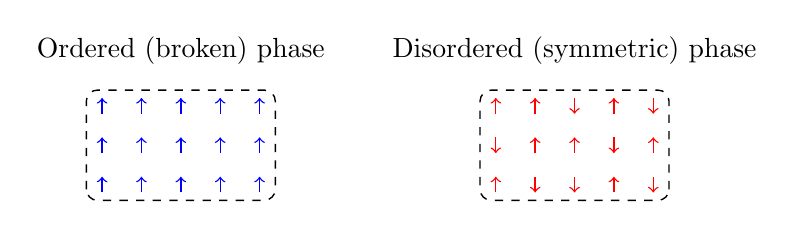
\begin{tikzpicture}
%\draw [dashed, blue, inner color=blue, outer color=white,
%fill opacity=0.4] 
%(0,1) circle (1.5);
%\node[text=blue] (n) at (-1.6,2.5)  {chain};
    \foreach \i in {5,...,9}
    \foreach \j in {1,...,3}
{
\draw [->, line width=0.5pt,blue] (-\i/2,0.2-\j/2) -- (-\i/2,0.4-\j/2);
}

\draw [dashed,line width=0.5pt, black, rounded corners]
        (-4.7,-1.4) rectangle (-2.3,0);
\node at (-3.5,0.5) {\alertb{Ordered (broken) phase}};

\draw [->, line width=0.5pt,red] (1/2,0.2-1/2) -- (1/2,0.4-1/2);
\draw [->, line width=0.5pt,red] (2/2,0.2-1/2) -- (2/2,0.4-1/2);
\draw [<-, line width=0.5pt,red] (3/2,0.2-1/2) -- (3/2,0.4-1/2);
\draw [->, line width=0.5pt,red] (4/2,0.2-1/2) -- (4/2,0.4-1/2);
\draw [<-, line width=0.5pt,red] (5/2,0.2-1/2) -- (5/2,0.4-1/2);
\draw [<-, line width=0.5pt,red] (1/2,0.2-2/2) -- (1/2,0.4-2/2);
\draw [->, line width=0.5pt,red] (2/2,0.2-2/2) -- (2/2,0.4-2/2);
\draw [->, line width=0.5pt,red] (3/2,0.2-2/2) -- (3/2,0.4-2/2);
\draw [<-, line width=0.5pt,red] (4/2,0.2-2/2) -- (4/2,0.4-2/2);
\draw [->, line width=0.5pt,red] (5/2,0.2-2/2) -- (5/2,0.4-2/2);
\draw [->, line width=0.5pt,red] (1/2,0.2-3/2) -- (1/2,0.4-3/2);
\draw [<-, line width=0.5pt,red] (2/2,0.2-3/2) -- (2/2,0.4-3/2);
\draw [<-, line width=0.5pt,red] (3/2,0.2-3/2) -- (3/2,0.4-3/2);
\draw [->, line width=0.5pt,red] (4/2,0.2-3/2) -- (4/2,0.4-3/2);
\draw [<-, line width=0.5pt,red] (5/2,0.2-3/2) -- (5/2,0.4-3/2);

\draw [dashed,line width=0.5pt, black, rounded corners]
        (2.7,-1.4) rectangle (0.3,0);
\node at (1.5,0.5) {\alert{Disordered (symmetric) phase}};

%       \filldraw [red] (0,0) rectangle ++(6pt,6pt); %circle (3pt);
%        \draw[thick,<->,gray] (0,-0.3)--(0,-0.8);
%        \draw [dashed,thick, black, rounded corners]
%        (-0.35,-1.8) rectangle (0+0.35,-0.9);
%        \filldraw[red!50!white, rounded corners]
%        (-0.35,-1.8) rectangle (0+0.35,-0.9);
%        \node at (0,-1.35) {$\mathcal{B}$};
\end{tikzpicture}
\end{figure}}
As example, we take the classical Ising model in which:
\begin{eqnarray} % \vec
&H = - J\,\sum_{\braket{i,\,\,j}}  S_i \cdot  S_j -  h \cdot \sum _i  S_i & \,\,,\\
&Z = \sum _{\{S_i\}} \, e^{-H/T} & \,\, ,
\end{eqnarray}
%where $\vec S_i$ is a d-dimensional vector with $\vec S_i \cdot \vec S_i = 1\,$. 
where $ S_i = \pm 1\,$ and $i,\,j$ indicate the sites of a $d$-dimensional lattice. 
%The system undergoes a CT driven by the temperature $T\,$ and described by the order parameter \alertb{$M=V^{-1}\sum _i  \braket{S_i}\,$} for $V\to +\infty\,$. 
\small{
\begin{figure}[!b]
\centering
\begin{tikzpicture}
\begin{axis} [width=8cm,height=3.2cm,xmax=1, axis lines=middle, enlargelimits,
xtick={0.5},ytick={0.},xticklabels={$T_c$},yticklabels={$ $}, xlabel=$T$,ylabel=$h$]
\draw [dashed, line width=0.5pt,gray] (50,-60) -- (50,60);
\node[text=blue] at (30,7) {\scriptsize{$M>0$}};
\node[text=blue] at (30,-8) {\scriptsize{$M<0$}};
\node[text=red] at (70,7) {\scriptsize{$M=0$}};
\node[text=red] at (70,-8) {\scriptsize{$M=0$}};
\node[text=red] at (70,-8) {\scriptsize{$M=0$}};
\addplot [domain=0:0.5,
samples=10,smooth,thick,black]
{0};
\filldraw [red] (49,-0.7) rectangle ++(3pt,3pt); %circle (3pt)
\end{axis}
\end{tikzpicture}
\end{figure}
}

\end{frame}


% With the characteristic length scale equal to infinity, we may guess that the structure of the correlations is the same at all length scales, i.e. the physics is invariant under a scaling transformation.

%%%%%%%%%%%%%%%%%%%%%%%%%%%%%%%%%%%%%%%%%%%%%%%%%%%%%%%%%%%%%%%%%%%%%%%%%%%%%%%%%%%%%%%%%%%%%%%%%%%%

\begin{frame}
\frametitle{Phase transitions and Critical phenomena}
\framesubtitle{Power-laws}
The CTs are characterized by power-law behavior:\\
$ $\\
\begin{itemize}
\item the correlation length $\xi$ defined as 
\[
\lim_{\abs*{i-j}\to \infty}\braket{ S_i \cdot S_j}\sim e^{-\abs*{i-j}/\xi}\,,
\]
scales as $\alertb{\quad \xi \sim \abs*{t}^{-\nu}}\,\,, \quad t = T/T_c -1 \,$;
\item the order parameter $M\,$: $\quad \alertb{ M \sim \abs*{t}^\beta}\,$;
\item the susceptibility $\chi = \sum _i \braket{ S_i \cdot S_j} \,$: $\quad \alertb{ \chi \sim \abs*{t}^{-\gamma}}\,$;
\end{itemize}
$ $\\
where the parameters $\nu\,,\,\,\beta\,,$ and $\gamma$ are called critical exponents.\\ 
$ $\\
%Since $\nu = 1$ for $d=2\,$, close to $T=T_c$ the correlation length diverges to $\infty\,$.
Close to the critical point, i.e. $t \to 0\,$, the correlation length diverges to $\infty\,$.
\end{frame}

%%%%%%%%%%%%%%%%%%%%%%%%%%%%%%%%%%%%%%%%%%%%%%%%%%%%%%%%%%%%%%%%%%%%%%%%%%%%%%%%%%%%%%%%%%%%%%%%%%%%

\begin{frame}
\frametitle{Phase transitions and Critical phenomena}
\framesubtitle{Renormalization group (RG)}

% With the characteristic length scale equal to infinity, we may guess that the structure of the correlations is the same at all length scales, i.e. the physics is invariant under a scaling transformation under which the coordinates change as $$$x → x = x/b, (4.1)$$$ where b is the rescaling factor. In other words, the basic structure of all correlations should be invariant under a transformation from the x to the x' coordinates. An example of this invariance appears in our result for the two-point correlation function C(x) ∼ x^{2−D} for x << ξ .

Close to critical point, the many-body system shows an universal critical behavior dependent only by few global properties:
\begin{itemize}
\item \alert{the space dimensionality $d\,$},
\item \alert{the nature and the symmetry of the order parameter},
\item \alert{symmetry-breaking pattern}.
\end{itemize}
$ $\\
$ $\\
These features are encoded in the \alertb{renormalization group (RG) theory} in which:
\begin{itemize}
\item we have a RG flow in the Hamiltonian space,
\item the critical points are described by the fixed points of the theory,
\item only a few perturbations are relevant, the corresponding positive eigenvalues are related to the critical exponents.
\end{itemize}
\end{frame}

%%%%%%%%%%%%%%%%%%%%%%%%%%%%%%%%%%%%%%%%%%%%%%%%%%%%%%%%%%%%%%%%%%%%%%%%%%%%%%%%%%%%%%%%%%%%%%%%%%%%

\subsection{Quantum transitions}

\begin{frame}
\frametitle{Quantum Transitions}
%\framesubtitle{Lindblad equation}
\textbf{\alertb{Quantum phase transitions}} are driven by the variation of the Hamiltonian parameters which determine the non-analytic behavior of the ground state.\\
$ $\\
In the large-volume limit, the \alertb{continuous quantum transitions} (CQT) are characterized by:
\begin{itemize}
\item a diverging correlation length: 
\begin{equation}
\alert{\xi \sim \abs*{\bar g}^{-\nu}} \,\,;
\end{equation}
\item a lowest energy gap $\Delta$ which vanishes:%qtime associated with a classic length l_c, so \xi_c \to \Delta
\begin{equation}
\alert{\Delta \sim \xi^{-z} \sim \abs*{\bar g}^{z\,\nu}} \,\,;
\end{equation}
\end{itemize}
where $\bar g = g - g_c$ is an Hamiltonian parameter which drives the quantum transition and $z$ is the dynamic critical exponent.
\end{frame}

\begin{frame}
	\frametitle{Quantum Transitions}
	\framesubtitle{Example - Quantum Ising model}
	
	As a paradigmatic model for quantum transitions, we consider the quantum Ising model whose Hamiltonian is given by:
	\begin{equation}
	\alert{
	  \hat H_{\rm Is} = -\sum_{x=1}^{L-1} \hat \sigma^{(1)}_x \hat
	  \sigma^{(1)}_{x+1} - g\, \sum_{x=1}^L \hat \sigma^{(3)}_x }\,\,,
	  \label{ising}
	\end{equation}
	where $\sigma^{(j)} _x$ are the Pauli matrices on the $x^{\rm th}$ site of the chain and $L$ is the system size.\\
	$ $\\
	
	The system undergoes a \alert{quantum transitions} at $\alert{g_c=1}\,$, between paramagnetic and ordered phases.\\
\end{frame}



%\section{Kitaev model}
\begin{frame}
	\frametitle{Kitaev Model}
	Kitaev Hamiltonian mapped into a spin-$1/2$ XY chain, by a 
	Jordan-Wigner transformation (OBC):
	$\qquad \qquad\alert{\hat c \longrightarrow \hat\sigma}\,$
	\begin{align}
		\label{KitaevH}
		\hat H _K^{\rm (ABC)} =- \sum _{x=1}^{L}\biggr[ \bigl(
		 \hat c_x^\dagger \, \hat c_{x+1} + 
		 \hat c_{x+1}^\dagger \,\hat c_x \bigl) + 
		 \delta\,\bigl( \hat c_x \, \hat c_{x+1} + 
		\hat c_{x+1}^\dagger \, \hat c_x^\dagger \bigl)\biggr] - 
		\sum _{x=1}^L  \mu \, \hat c_x^\dagger \, \hat c_{x}  \,\,;
	\end{align}
	\begin{figure}[!h]
		\centering
		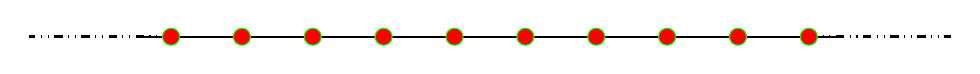
\begin{tikzpicture}[scale=0.9]
			\draw [-, line width=0.8pt, black] (-5.5,0.5) -- (4.5,0.5);

			\draw [dash dot dot, line width=1.2pt, black] (-5,0.5) -- (-7,0.5);
			\draw [dash dot dot, line width=1.2pt, black] (4,0.5) -- (6,0.5);

			\fill [red, draw=green] (-5,0.5) circle (0.12);
			\fill [red, draw=green] (-4,0.5) circle (0.12);
			\fill [red, draw=green] (-3,0.5) circle (0.12);
			\fill [red, draw=green] (-2,0.5) circle (0.12);
			\fill [red, draw=green] (-1,0.5) circle (0.12);
			\fill [red, draw=green] (4,0.5) circle (0.12);
			\fill [red, draw=green] (3,0.5) circle (0.12);
			\fill [red, draw=green] (2,0.5) circle (0.12);
			\fill [red, draw=green] (1,0.5) circle (0.12);
			\fill [red, draw=green] (0,0.5) circle (0.12);
			%\node (n) at (-4.5,0.85)  {$\bm{\hat c_1} $};
			%\node (n) at (4.5,0.95)  {$\bm{\hat c_L^\dagger} $};
		\end{tikzpicture}
	\end{figure}

	\alert{\bf Continuous Transition point:} 
	\begin{align}
		\mu _c = -2 \qquad {\rm and} \qquad \delta = 1 \,\,{\rm fixed} \,\,;\notag
	\end{align}
	\alert{RG dimensions}:	
	$ $\\
	\begin{align}
		w = \mu - \mu_c \longrightarrow y_w = 1 \qquad 
		\hat c_x \, ,\,\, \hat c_x^\dagger \longrightarrow y_c = 1/2 \qquad
		{\rm dynamic \,\, exp:\,\,} z =1
		\,\,.\notag
	\end{align}
	
\end{frame}


\subsection[FSS]{Finite Size Scaling (FSS) at the equilibrium}

\begin{frame}
\frametitle{Finite Size Scaling (FSS) at the equilibrium}
\framesubtitle{Kitaev model}
\small
At the critical point, the \alert{ground state} $\ket{0}\bra{0}$ correlation function:
\begin{equation}
%\begin{subequations}
\label{correlations}
%\begin{align}
\alertb{
G_c(x,y,t)}  \alertb{ =  
\braket{0 \big| \hat c_{x}^\dagger \hat
  c_{y}^{\phantom\dagger} + \hat c_{y}^\dagger \hat
  c_{x}^{\phantom\dagger} \big| 0}}\,\,,%\label{ctf}
%\alertb{G_p(x,y,t)} & \alertb{= {\rm
%  Tr}[\rho(t) (\hat c_{x}^\dagger \hat c_{y}^\dagger + \hat
%  c_{y}^{\phantom\dagger} \hat c_{x}^{\phantom\dagger})]}\,\,.
%\end{align}
%\end{subequations}
\end{equation}
satisfies for $L\to \infty\,$ and using RG theory:
\begin{equation}
\alert{
G_{c}(x,y,\bar \mu)= b^{-2y_c} \,\mathscr{G}_{c} \left( x/b, y/b, \bar \mu \,b^{y_\mu}\right)} \,\,,
\end{equation}
where $y_\mu=1\,,\,\,y_c=1/2$ are the RG dimensions of, respectively, the parameter $\mu$ and the fermionic operator $\hat c_x$ and $\hat c_x^\dagger\,$.\\
$ $\\
$ $\\
$ $\\
If the system size $L$ is finite \alert{$\Longrightarrow$} in the FSS limit, i.e. when we keep the ratio \alertb{$\xi / L\,$} fixed for $L \to \infty$; in other words, when wee fix \alertb{$b=L$}, we have:
\begin{eqnarray}  
\label{scalKitaev}
\alert{
G_{c}(x,y,\bar \mu; L)= L^{-1} \,\Bigr[\mathscr{G}_{c} \left( X, Y, \kappa\right) + O(L^{-1}) \Bigr]} \,\,,\\
\alertb{X \equiv x/L}\,, \qquad \alertb{Y \equiv y/L}\,, \qquad \alertb{\kappa = \bar \mu \,L^{y_\mu} }\,\,.
\end{eqnarray}

\end{frame}

   %\input{slides/model}
   \section{PART I}

\begin{frame}
	\frametitle{\Large{\rm PART I}}

\begin{center}
	{\LARGE{ \bf Round - Trip}\\}
	\medskip
	\medskip
	\medskip
	\texttt{ \Large
  FT, E. Vicari PR B {\bf 105}, 235124 \\ 
  FT, S. Scopa PR B {\bf 108}, 104316 }
\end{center}
\end{frame}

\section{KZ Protocol}

\begin{frame}
	\frametitle{Kibble Zurek(KZ) Protocol}
	\begin{itemize}
		\item[(i)] 
			Start at the equilibrium state (classical) and at the 
			\\ground state 
			$\ket{\Psi(t = t_i)} \equiv \ket{\Psi(w_i < 0 )}\,$ (quantum);
	\bigskip
	\bigskip
		
			\begin{columns}
				\begin{column}{0.4\textwidth}
			\item[(ii)] quantum case:
			\begin{align}
				\frac{ d \ket{ \Psi(t) } }{dt} = - i \hat H[w(t)] \ket{\Psi(t)} 
				\,\,; \notag
			\end{align}
				\end{column}
				\begin{column}{0.4\textwidth}
			\item[(ii)] classical one:	\\ $ $\\
			\alertb{\tt Metropolis algorithm};
				\end{column}
			\end{columns}
			\begin{align}
				& \alert{\Downarrow} \notag \\
				\alert{w(t)} &\alert{= t/t_s} \,\,; \notag
			\end{align}
			from $w_i < 0$ to $w_f > 0\,$, where $t_s$ is the time 
			scale of the slow variations of $w\,$.
	\bigskip
	\bigskip
	
		\item[(iii)] Then, for $t > t_f$, $w(t)$ decreases with the same
		  $t_s$ , from $w_f >0$ to the original value 
		 $wi < 0\,$, closing the cycle.
	\end{itemize}
\end{frame}

   \section{Observables}

\begin{frame}
	\frametitle{Observables}

	\begin{center}
	\alertb{\bf Classical Ising model}
	\begin{align}
		&M(t) = \frac{1}{L^2} \sum_{i} \braket{S_i}_t \,\,; \\
		&G(t,{\bm x},{\bm y}) \equiv \langle s_{\bm x}\, s_{\bm y}\,
		\rangle_t \,.
	\end{align}
	\end{center}
	\begin{center}
	\alertb{\bf Quantum models}\\
	Adiabaticity function:
	\begin{eqnarray}
  		A(t) = \Big|\braket{ \Psi_0[w(t)] | \Psi(t) }\Big|\,;
  		\label{adtfunc}
	\end{eqnarray}
	\end{center}
	
	%\begin{columns}
	%\begin{column}{0.5\textwidth}
	%\begin{center}
	%{\bf Ising:}
	%\begin{align}
	%	M(t) \equiv {1\over L} \sum_x  \langle \Psi(t) | \, \sigma_x^{(1)}
	%	| \Psi(t) \rangle\,;
	%	\notag
	%\end{align}
	%\end{center}
	%\end{column}
	%\begin{column}{0.4\textwidth}
	\begin{center}
	{\bf Kitaev:}
	\begin{align}
		C(x,t)  \equiv  \langle \Psi(t) |
  		\, c_j^\dagger c_{j+x} 
  		+ c_{j+x}^\dagger c_{j} \, | \Psi(t) \rangle \, \, . \notag
	\end{align}
	\end{center}
	%\end{column}
	%\end{columns}
	
	
\end{frame}

   \subsection{Dynamic scaling}

\begin{frame}
	\frametitle{Dynamic scaling framework for the round-trip}
	The asymptotic dynamic FSS behavior is obtained by taking 
	$t_s \to \infty$ and $L \to \infty\,$:
	\begin{eqnarray}
  		&K = w(t) L^{y_w}\,, \qquad &\Upsilon = t_s/L^{\zeta}\,,  
  		\label{KZscavar}\\
 		 &\Theta_i
 		 = w_i\, t_s^{1-\kappa} \,,\qquad &\Theta = w(t) \,
  		t_s^{1-\kappa} = t / t_s^{\kappa} \,,\nonumber
	\end{eqnarray}
	where
	\begin{eqnarray}
		\zeta = y_w + z\,,\qquad 
		\kappa = {z/\zeta} \,,\qquad
		1-\kappa = {y_w/\zeta}\,.\label{KZexps}
	\end{eqnarray}
	with $w_f = - w_i = w _\star$, we have:
	\begin{eqnarray}
  		\Upsilon = t_s/L^{\zeta}\,, \quad
  		\Theta = w(t) \, t_s^{1-\kappa}\,,\quad
  		\Theta_\star =  w_\star\, t_s^{1-\kappa} \,\,.
 		\label{scalvar2}
  	\end{eqnarray}
\end{frame}




\section{Numerical results}


\subsection{Classical Ising}

\begin{frame}
	%\frametitle{$\qquad \qquad \qquad M^{(a/b)}(t,t_s,w_\star,L) 
	%			\approx L^{-y_l} {\cal M}_i(\Upsilon,\Theta, \Theta_\star)$}
	\frametitle{Numerical results - Classical Ising}
	
	%\begin{align}
	%	M(t,t_s,w_i,L) \approx L^{-y_l} {\cal M}_i(\Upsilon,\Theta)\,\,.
	%\end{align}
	\begin{columns}
	\begin{column}{0.52\textwidth}
	\begin{figure}[!htb]
  		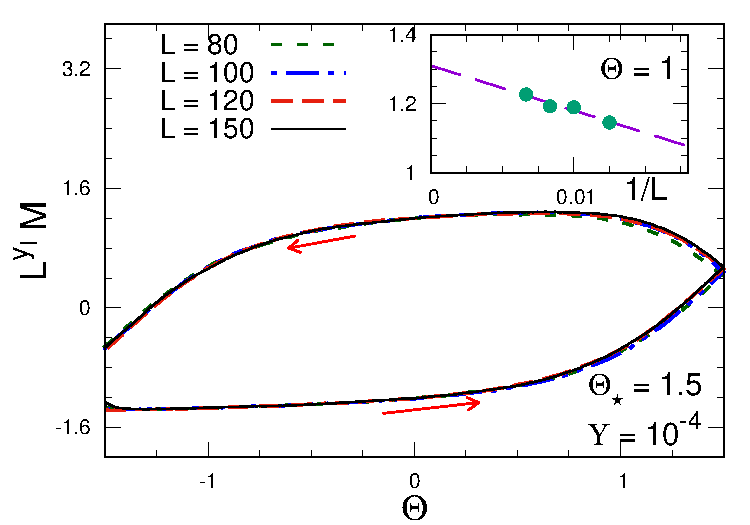
\includegraphics[width=1.\columnwidth]{paper/isC2DT15Y104.pdf}
  		
  		\caption{ \alert{$M^{(a/b)}(t,t_s,w_\star,L) 
				\approx L^{-y_l} {\cal M}_i(\Upsilon,\Theta, \Theta_\star)$}
				$\Upsilon=10^{-4}$, fixed $\Theta_\star =
    				1.5$ and plotted versus $\Theta=w(t) t_s^{1-\kappa}$.  }
  		\label{roundtripM}
	\end{figure}
	\end{column}
	\begin{column}{0.5\textwidth}
	
	\begin{figure}[!htb]
    		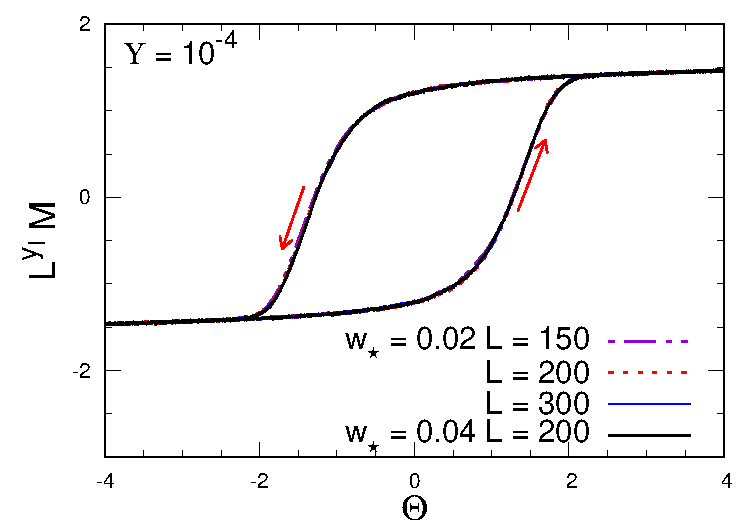
\includegraphics[width=1.\columnwidth]{paper/isC2Dw002Y104.pdf}
  		\caption{ Thermalized classical state for
    		fixed $\Upsilon=10^{-4}$, and fixed $w_\star = 0.02$ and $w_\star
    		= 0.04$. $\qquad \qquad \qquad \qquad \qquad \qquad \qquad \qquad$}
  		\label{roundtripMW}
	\end{figure}
	\end{column}
	\end{columns}
	
\end{frame}



\begin{comment}
\subsection{Quantum Ising}

\begin{frame}
	
	\frametitle{Numerical results - Quantum Ising}
	\begin{columns}
	\begin{column}{0.52\textwidth}
	\begin{figure}[!htb]
		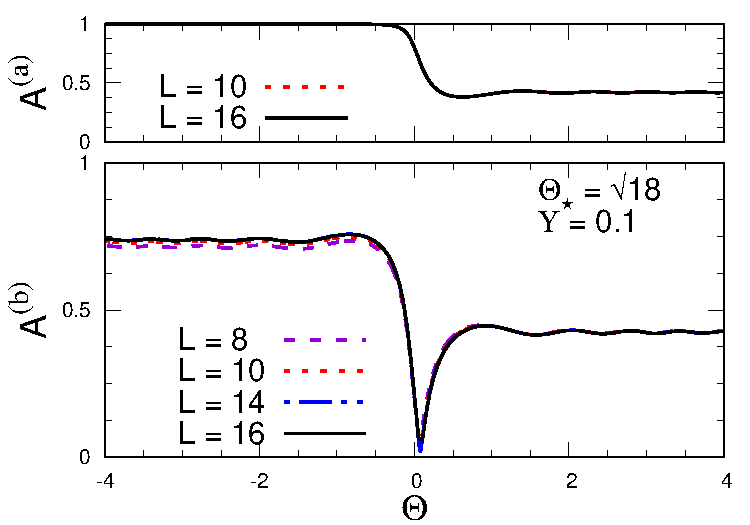
\includegraphics[width=1\columnwidth]{paper/headIQMY01ThA.pdf}
		\caption{ \alert{$ A^{(a/b)}(t,t_s,w_\star,L) \approx 
 				{\cal A}^{(a/b)}(\Upsilon,\Theta,\Theta_\star)\,\,$};
		fixed $\Upsilon = t_s/L^\zeta= 0.1$ and $\Theta_\star = w_\star
  		L^{1-\kappa}=\sqrt{18}$, for the outward (top) and return (bottom). }
    		\label{roundtripA}
	\end{figure}
	
	\end{column}
	\begin{column}{0.5\textwidth}
	
	\begin{figure}[!htb]
		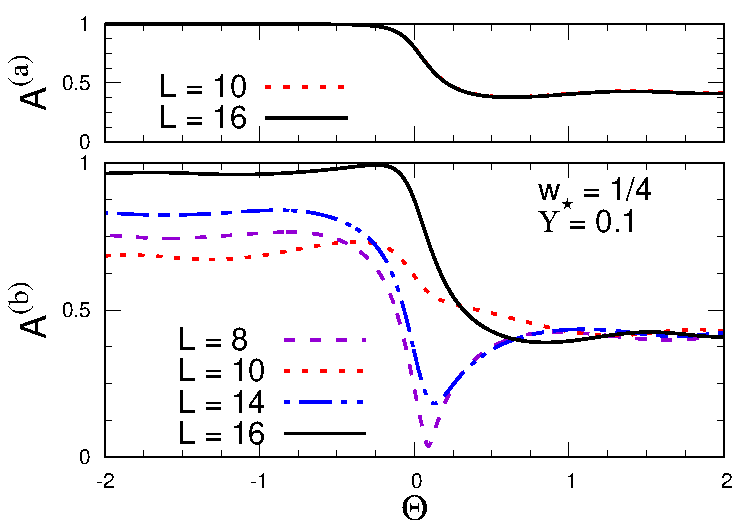
\includegraphics[width=1\columnwidth]{paper/headIQMY01W025A.pdf}
  		\caption{ Fixed $\Upsilon = 0.1$ and $w_\star = 1/4$, for the outward 
  		(top) and return (bottom), versus $\Theta=w(t)L^{1-\kappa}$.
  		$\qquad \qquad \qquad \qquad \qquad \qquad \qquad \qquad$}
  		\label{roundtripAW}
		\end{figure}
	\end{column}
	\end{columns}

\end{frame}
\end{comment}


\subsection{Kitaev chain}

\begin{frame}
	
	\frametitle{Numerical results - Kitaev chain}
	
	\begin{columns}
	\begin{column}{0.52\textwidth}
		\begin{figure}[!htb]
			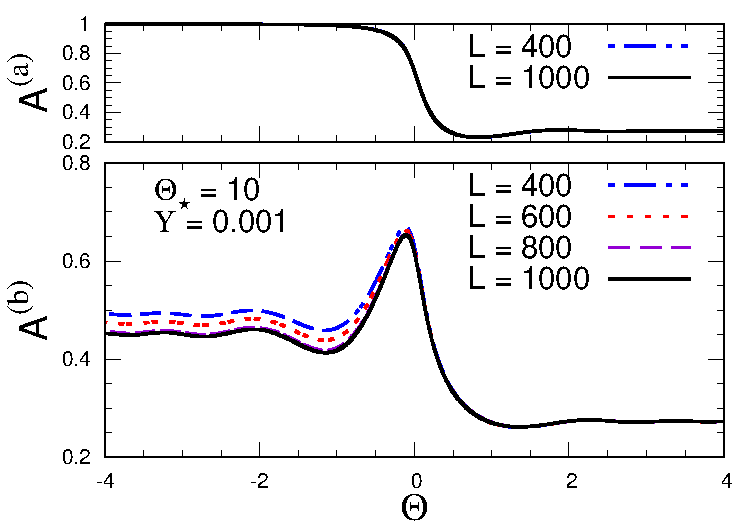
\includegraphics[width=1\columnwidth]{paper/headKITY0001Th10A.pdf}
  			\caption{ \alert{$ A^{(a/b)}(t,t_s,w_\star,L) \approx 
 				{\cal A}^{(a/b)}(\Upsilon,\Theta,\Theta_\star)\,\,$};
  			Finite $\Theta_\star=10$ at fixed $\Upsilon =t_s/L^\zeta = 0.001$
  			and $\Theta_\star = w_\star L^{1-\kappa}=10$, for outward
  			 and return.
    $\Theta$, }
  			\label{roundtripdfssE}
		\end{figure}
	
	\end{column}
	\begin{column}{0.5\textwidth}
	
	\begin{figure}[!htb]
  		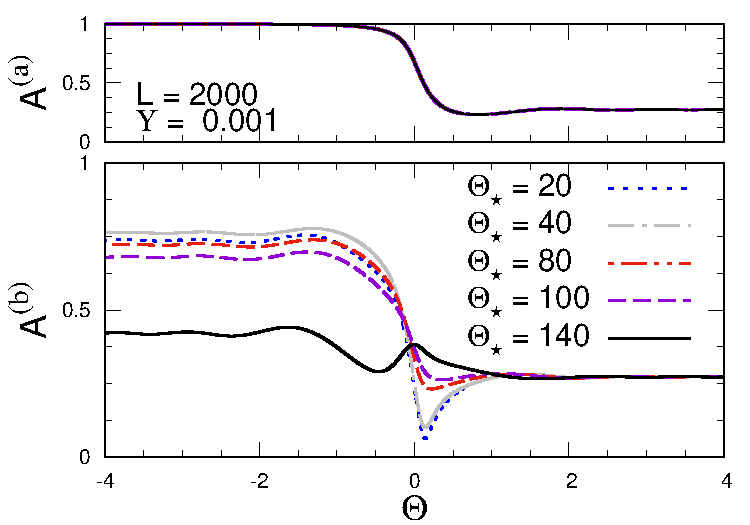
\includegraphics[width=1\columnwidth]{paper/headKITY0001L2000A.pdf}
 		\caption{At $L=2000$ and $\Upsilon = 0.001$ for the outward (top)
 		 and return (bottom), versus $\Theta$, for various 
 		 $\Theta_\star$. $\qquad \qquad \qquad \qquad \qquad \qquad \qquad \qquad \qquad \qquad \qquad \qquad \qquad \qquad \qquad \qquad$}
 		 %=w(t)L^{1-\kappa}
  \label{diffThetaStarA}
\end{figure}

	\end{column}
	\end{columns}


\end{frame}

   \subsection{Limit $\Theta_\star \to \infty$}

\begin{frame}	
	\frametitle{The limit $\Theta_\star \to \infty$}

		\begin{figure}
   			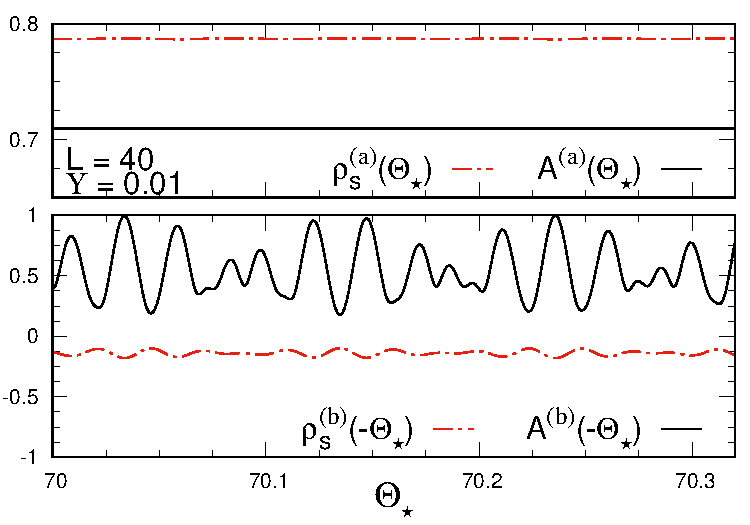
\includegraphics[width=7.5cm]{paper/diffThstaru001T70l40.pdf}
  			\caption{ {\bf Kitaev} - Fixed $L = 40$, $\Upsilon = 0.01$ versus
    			$\Theta_\star$, close to $\Theta_\star = 70$.  The top plot shows 
    			the
    			values at $\Theta=\Theta_\star$, while the bottom
    			 at $\Theta=-\Theta_\star$, with the particle density $\rho_s = \bra{\Psi(t)}  c^\dagger_x c_x \ket{\Psi(t)} - \rho_{\rm critical-gs}$. }
			\label{roundtripDiffThetaAR}
		\end{figure}

	%\end{column}
	%\end{columns}
\end{frame}

\begin{comment}
	\begin{columns}
	
	\begin{column}{0.52\textwidth}
		\begin{figure}[!htb]
			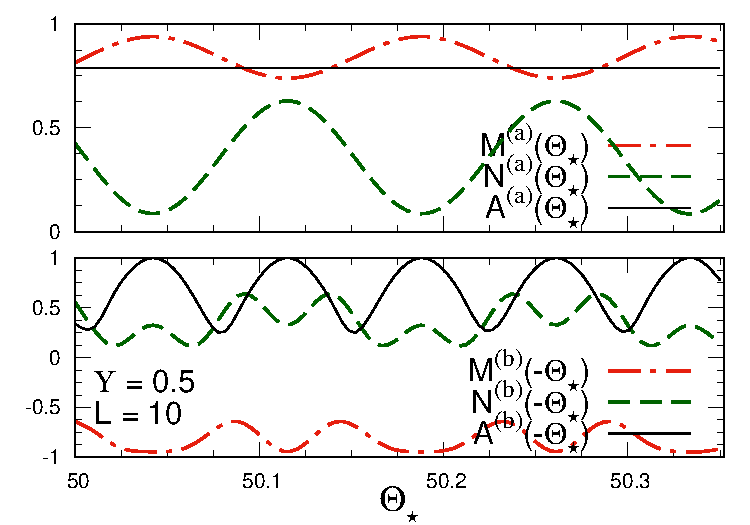
\includegraphics[width=1\columnwidth]{paper/diffThstaru50s50l10.pdf}
 			\caption{ {\bf Ising} - Fixed $L = 10$, $\Upsilon = 0.5$ versus $
 			\Theta_\star$,
 			 close to $\Theta_\star = 50$. The top plot shows the values at 
 			 $\Theta=\Theta_\star$, while the bottom plot the values 		
 			 at $\Theta=-\Theta_\star$. }
			\label{roundtripDiffTheta}
		\end{figure}
	\end{column}
\end{comment}
	%\begin{column}{0.5\textwidth}


\section{Two-Level Model}

\begin{frame}
	
	\frametitle{Two-Level Model:	$\qquad \qquad H_{2\ell}(t) = - \beta(t) 
				\sigma^{(3)}+ {\Delta\over 2} \sigma^{(1)}$}
	
	\begin{columns}
	\begin{column}{0.52\textwidth}
		\begin{figure}[!htb]
  			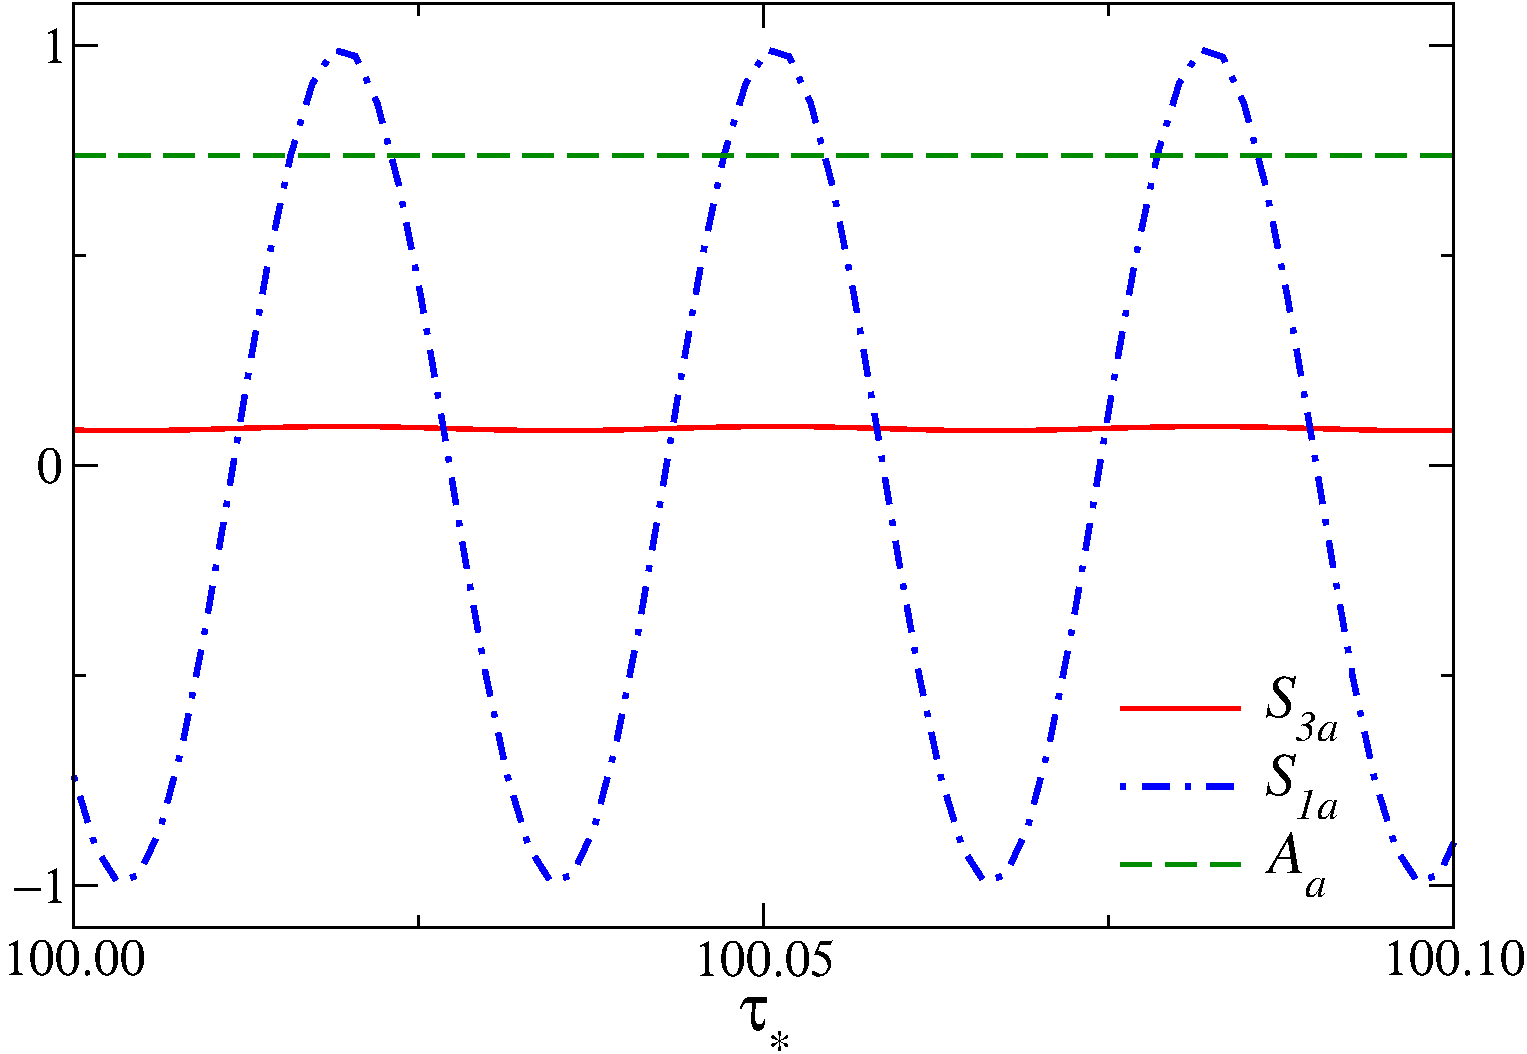
\includegraphics[width=1\columnwidth]{paper/oscillationa.pdf}
  			\caption{Dependence on $\tau_\star\equiv t_\star/\sqrt{t_s}$ at 
  			the end of the first dynamic branch for $\upsilon=1$, 
  			and $\tau_\star\approx 100$.}
 		 	\label{lzfigs}
		\end{figure}
	
	\end{column}
	\begin{column}{0.5\textwidth}
		\begin{figure}[!htb]
			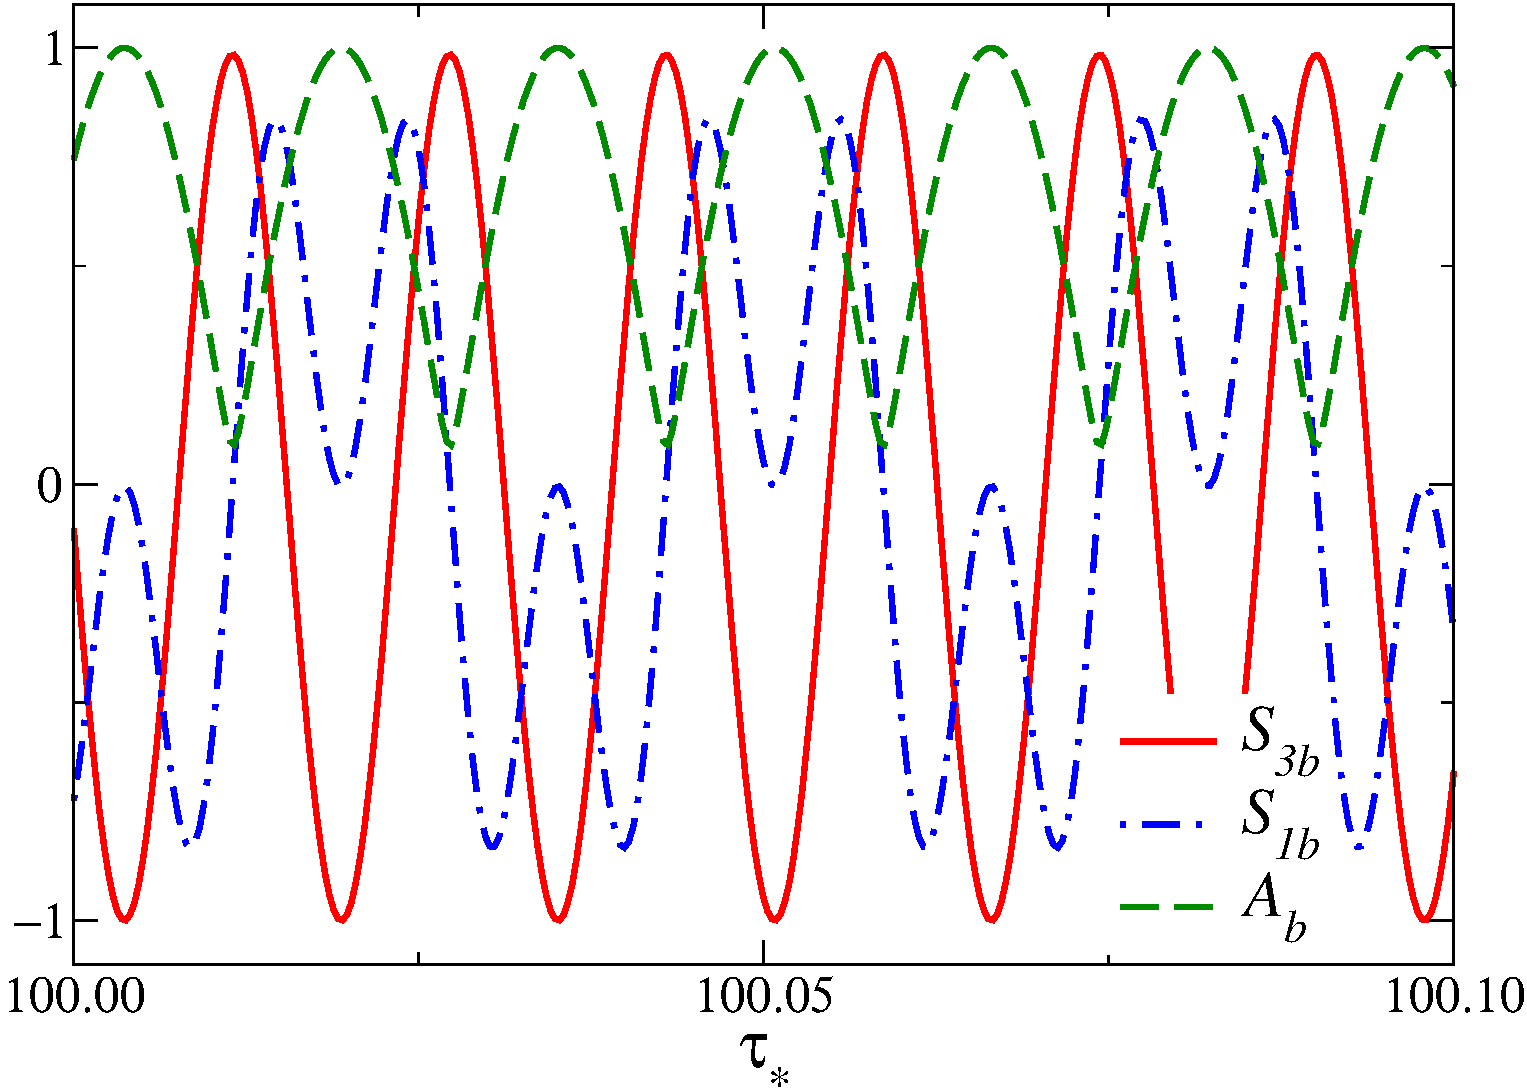
\includegraphics[width=1\columnwidth]{paper/oscillationc.pdf}
  			\caption{Dependence on $\tau_\star$ at the end of round-trip 
  			protocol for $\upsilon= t_s \Delta^2 =1$, and 
  			$\tau_\star\approx 100$.}
  			\label{lzfigs}
		\end{figure}


	\end{column}
	\end{columns}


\end{frame}

   \begin{frame}
	%\frametitle{$\qquad \qquad \qquad M^{(a/b)}(t,t_s,w_\star,L) 
	%			\approx L^{-y_l} {\cal M}_i(\Upsilon,\Theta, \Theta_\star)$}
	\frametitle{First Order Quantum transition (FOQT)}

    \begin{equation}
        \label{eq:model}
        \hat{H}(h_\perp,h_\parallel)=-J\sum_{j=1}^{L-1} \hat\sigma^{(3)}_j\hat\sigma^{(3)}_{j+1} -\sum_{j=1}^L (h_\perp\hat\sigma^{(1)}_j + h_\parallel \hat\sigma^{(3)}_j).   
    \end{equation}
        
    \begin{center}
		\begin{figure}
					   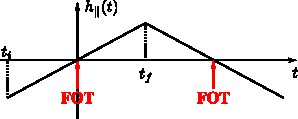
\includegraphics[width=8.4cm]{paper/protocol_foqt.pdf}
					  \caption{ FOQT Round-trip Protocol where we keep $h_\perp$ fixed and $h_\parallel (t) = t / t_s$.}
					\label{protocol_foqt}
		\end{figure}
	\end{center}
	
	
	
\end{frame}

\begin{frame}
    \frametitle{Out-Of-Equilibrium FSS at FOQT }

    Degeneracy of the 2 lowest energy level for finite $L$ approaching the FOQT point $\longrightarrow$ Two-levels model\\
    $ $\\

    We formulate the OFSS regime as the limit $L \to \infty$, $u = t_s L^{-1} M_0^{-1} \to \infty$.\\
    $ $\\
    The time-dependent expectation values of local observables are proportional to quasi-universal OFSS functions of the variables:
    \begin{align}
        \tau &= \frac{t}{\sqrt{u}} \,\,,\\
        \upsilon &= u \,\,\Delta^2(h_\perp, L) \,\,. 
    \end{align}

\end{frame}

\begin{frame}
    \frametitle{Validity of our scaling hypothesis}




    %\begin{align}
	%	M(t,t_s,w_i,L) \approx L^{-y_l} {\cal M}_i(\Upsilon,\Theta)\,\,.
	%\end{align}
	\begin{columns}
        \begin{column}{0.52\textwidth}
            \begin{figure}[t]
                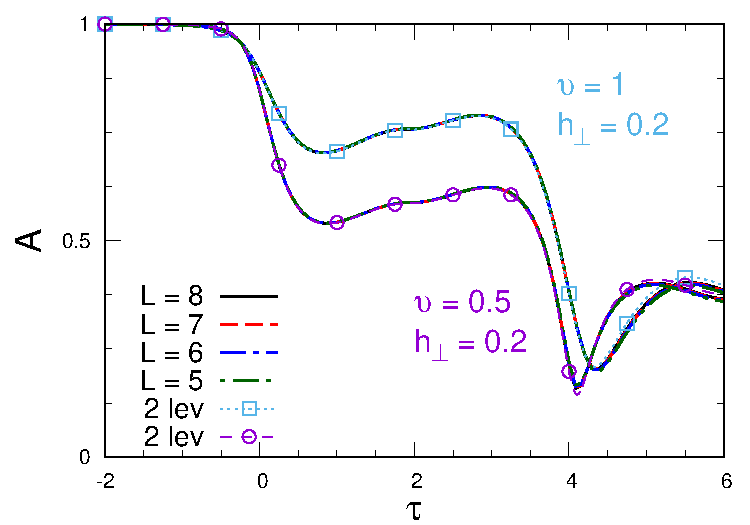
\includegraphics[width=1.\columnwidth]{paper/tripAt2u05g02-new.pdf}
                \caption{OFSS  of the adiabaticity function in $A(h_\perp,t,t_s,L)\sim {\cal F}_A(\tau,\upsilon)$ shown as a function of the rescaled time $\tau$ during a round-trip protocol with $|\tau_i|=\tau_f =2$ (FOTs at $\tau=0,4$).}
                \label{AtripAt2u05g02}
            \end{figure}
        \end{column}
        \begin{column}{0.5\textwidth}
            \begin{figure}[t]
                \centering
                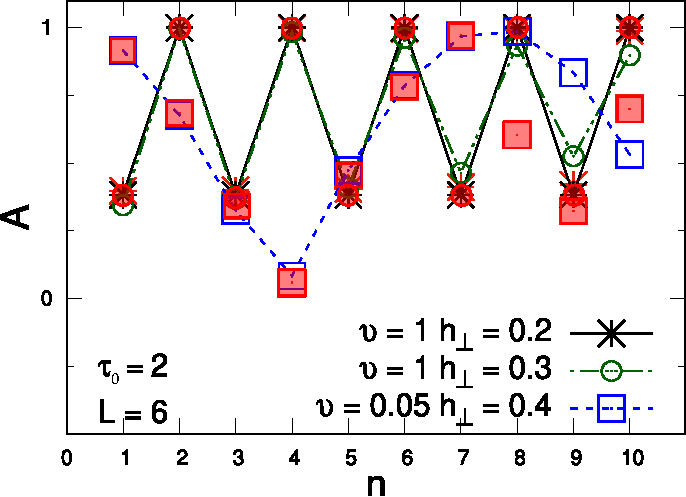
\includegraphics[width=1.\columnwidth]{paper/strobA.pdf}
                \caption{Stroboscopic evolution of $A$  as function of  $n$ (corresponding to times $t=t_0(4n-1)$) at fixed $L=6$, $\tau_0=2$}\label{fig:strobo}
            \end{figure}
        \end{column}
        \end{columns}
\end{frame}


\begin{frame}
    \frametitle{ Effective description in the OFSS regime}

    Emergence of an effective two-level description which involves the lowest two states near the FOT. \\
    $ $\\
    With this effective description, we reduce the driving protocol to a series of LZS and we determine an analytical expression of the OFSS functions:
    \begin{align}
        {\cal F}_A(\tau,\upsilon)
        \nonumber
        &=e^{-\frac{\pi\upsilon}{32}}\Bigg|\sqrt{\frac{1}{2}+ \frac{|\tau|}{\sqrt{4\tau^2+\upsilon}}} \mathscr{D}_{\frac{i u}{8}}(\sqrt{2}e^{i\frac{3\pi}{4}}\tau) 
        \nonumber\\
        &\quad -\frac{\sqrt{\upsilon} e^{-\frac{i\pi}{4}}}{2\sqrt{2}} \sqrt{\frac{1}{2}- \frac{|\tau|}{\sqrt{4\tau^2+\upsilon}}} \mathscr{D}_{-1+\frac{i u}{8}}(\sqrt{2}e^{i\frac{3\pi}{4}}\tau)\Bigg|
    \end{align}

    $ $\\
    {\bf Breakdown of the effective description}\\

    Corrections to the scaling behavior are expected when:
    \begin{align}
        \tau   \gtrsim O(t_{KZ}) 
        \qquad {\rm with} \qquad
        t_{KZ} & = \sqrt{u} \,\,.
    \end{align}

\end{frame}
   \section{PART II}

\begin{frame}
	\frametitle{\Large{\rm PART II}}

\begin{center}
	{\LARGE{ \bf Dissipation}\\}
	\medskip
	\medskip
	\medskip
	\texttt{ \Large
  A. Franchi, FT PR B \textbf{108}, 094114 (2023) }
\end{center}
\end{frame}

\section{Dissipation}
	\subsection{Lindblad framework}

\begin{frame}
	\frametitle{Lindblad framework}
\ba{eqlindblad}
        \frac{d\rho}{dt} = {\cal L}[\rho] =
                -i \Bigr[ H, \rho \Bigr] + \mathbb{D}[\rho] \pc
\ea

${\cal L}$ is the Liouville superoperator, and $\mathbb{D}$ is the 
dissipation term with coupling $w$:
\ba{dissipator}
        \mathbb{D}[\rho] = & w \sum_{x \in {\cal I}}
                \mathbb{D}_x[\rho] \cm \\
        \mathbb{D}_x[\rho] = &
                \hat L_x \rho \hat L_x^\dagger -
                \frac{1}{2} \Bigl\{ \rho, \hat L^\dagger_x \hat L_x \Bigl\} \pc
\ea
	

\end{frame}


\begin{frame}
\frametitle{Sunburst geometry}

\begin{figure}
    \centering
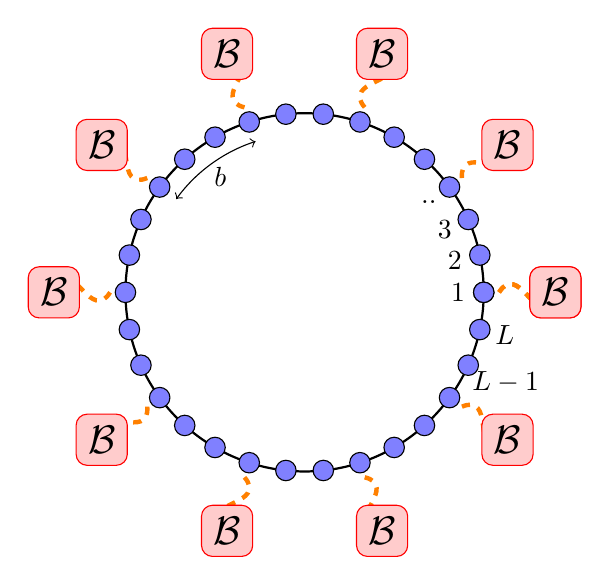
\begin{tikzpicture}[scale=0.65]
    \draw[thick] (0,0) circle (3.5cm);

    \foreach \x in {0,12,...,360}
    \filldraw [fill=blue!50] (\x:3.5cm) circle (0.2);

    \foreach \x in {0,36,...,360}
    \draw[orange, dashed, ultra thick] (\x:3.8cm) .. controls (\x+8:4.2cm) and (\x-8:4.6cm) .. (\x:4.6cm);

    \foreach \x in {0,36,...,360}
    \node[rectangle,
    draw = red,
    text = black,
    fill = red!20!white,
    rounded corners,
    minimum size=0.65cm] (r) at (\x:4.9cm) {\Large $\mathcal{B}$};

    \draw[<->] (108:3.1cm) arc
    [start angle=108,
        end angle=144,
        radius=3.1cm,
    ] ;

    \node[] (s1) at (126:2.8cm) {$b$};

    \node[] (s1) at (0:3cm) {$1$};
    \node[] (s2) at (12:3cm) {$2$};
    \node[] (s3) at (24:3cm) {$3$};
    \node[] (s4) at (36:3cm) {$..$};
    \node[] (s5) at (-12:4cm) {$L$};
    \node[] (s6) at (-24:4.3cm) {$L-1$};
\end{tikzpicture}
    \caption{Sketch of a Kitaev ring with $L=30$ qubits coupled with $n=10$ dissipators in a \textit{sunburst} geometry ($b=3$ in the figure).}
    \label{fig_sketch_sunburst_dissipation}
\end{figure}


\end{frame}


\begin{frame}
	\frametitle{Liouvillian gap}

\ba{eigencalL}
        \widetilde{\cal L}[\widetilde \rho_i] = \lambda_i \widetilde \rho_i \cm
        \qquad \lambda_i \in \numberset{C} \pc
\ea

\be{vecrho}
        \rho_{ij} \ket i \bra j  \longrightarrow  \widetilde \rho_{ij} \ket i \ket j \pt
\ee

\ba{vecteqlindblad}
        \widetilde{\mathcal{L}} =& -i \big(\hat{H} \otimes \hat{\mathbb{I}}
                - \hat{\mathbb{I}}\otimes \hat{H}^t \big) +
                w\sum_{x \in {\cal I}}\hat{L}_{x}\otimes \hat{L}^*_{x}\\
        &-\frac{w}{2}\sum_{x \in {\cal I}}\big(\hat{L}^{\dagger}_{x}\hat{L}_{x}
                \otimes\hat{\mathbb{I}}+\hat{\mathbb{I}}
                        \otimes\hat{L}^t_{x}\hat{L}^*_{x}\big) \pt
\ea

\ba{Lioulliangap}
\Delta_{\lambda} = - \max_{i} {\rm Re}{\lambda_i } \pt
\ea


\end{frame}


\begin{frame}
	\frametitle{Interplay between local and homogeneous dissipation}
	The number of the external baths:
	\be{}
		n \equiv L / b \pc
	\ee
	$ $\\
	\vspace{0.5cm}
	$b$ fixed  $\longrightarrow$ local dissipation with 
	$\Delta_\lambda \sim L^{-1} f(\mu, wL) 
	\qquad L\to\infty \pc$\\
	\vspace{1cm}
	$n$ fixed $\longrightarrow$ homogeneous dissipation with
	$\Delta_\lambda \sim L^{-3} \tilde{f}(\mu, w)
	\qquad L\to\infty\,\,$.
\end{frame}

\begin{frame}
	\frametitle{Liouvillian gap $b$ fixed}
\begin{figure}[!h]
    \centering
    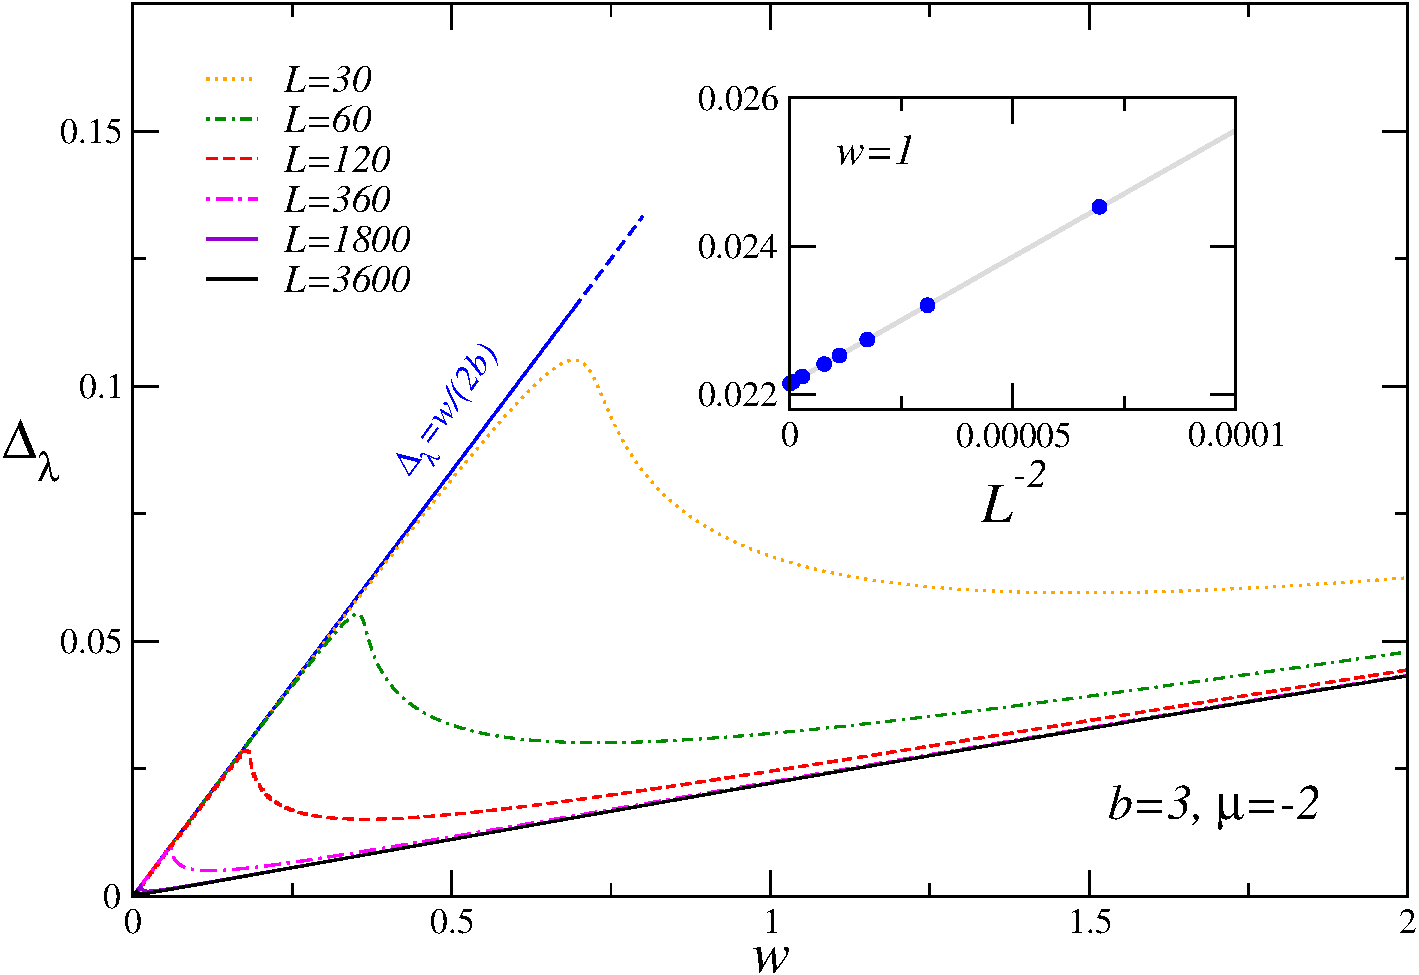
\includegraphics[width=6.4cm]{imm/gapliouv3b.pdf}
	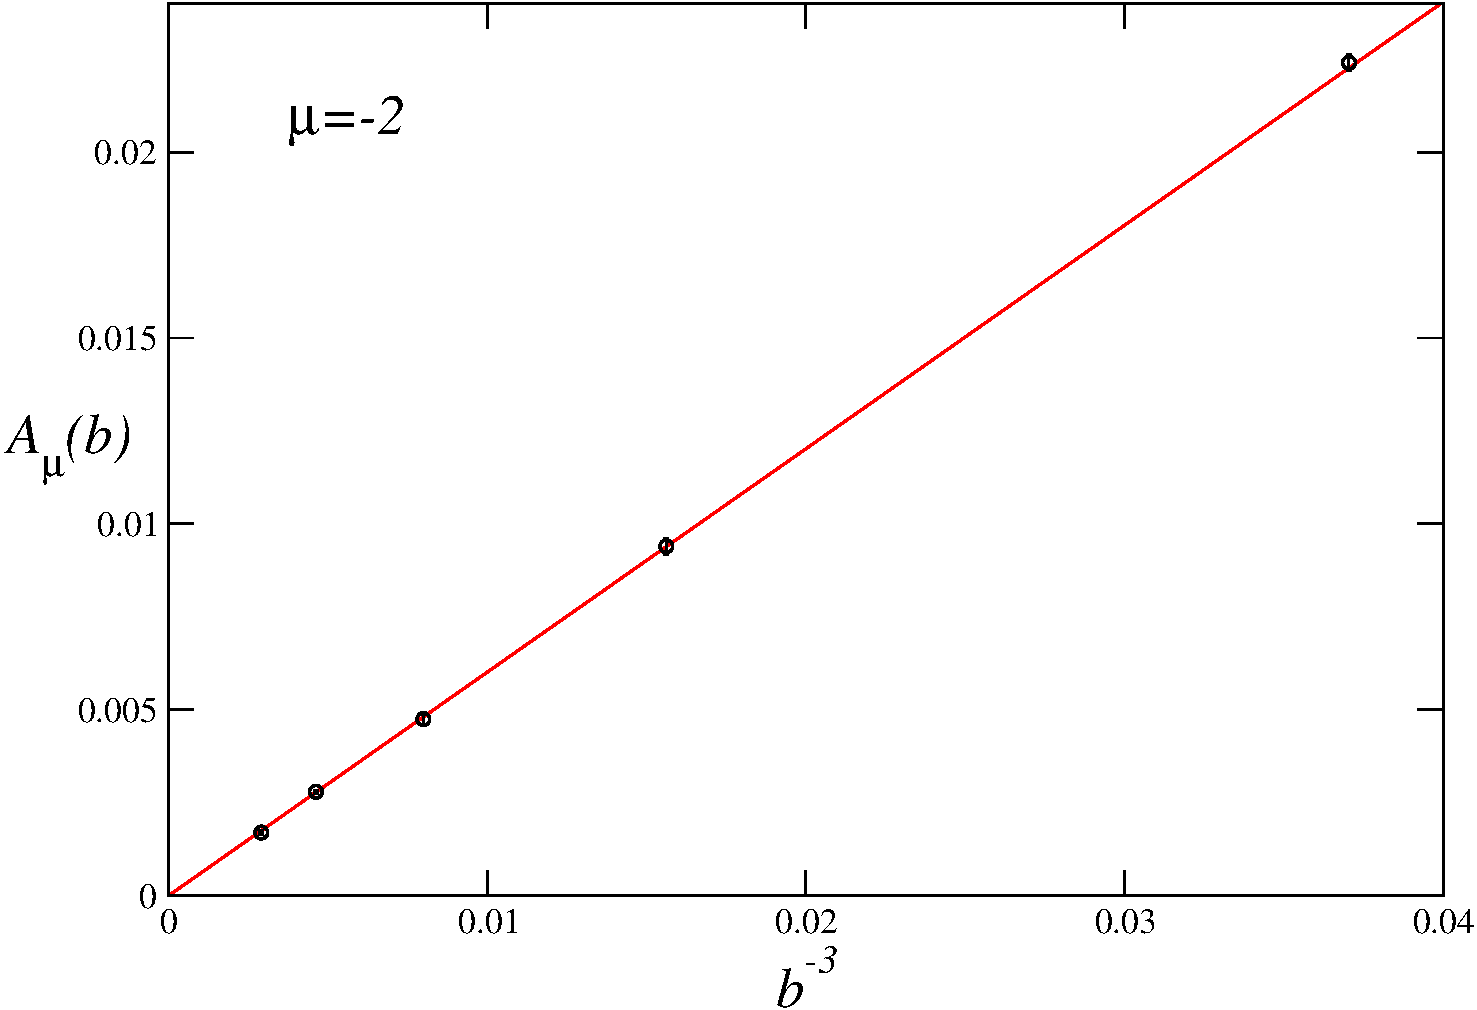
\includegraphics[width=6.4cm]{imm/ratelatetime.pdf}
    \caption{Liouvillian gap $\Delta_\lambda$ in terms of the dissipation coupling $w$ for $b=3$ and fixed $\mu=-2$.}
    \label{fig_liouvgap3b}
\end{figure}
\begin{equation}
    \Delta_\lambda(w, b)=A_\mu(b) w\,,\quad A_\mu(b)=\frac{C_\mu}{b^{3}}\,,\quad w>w_*\,,
    \label{eq_liouvillian_gap_largeL}
\end{equation}
\end{frame}

\begin{frame}
	\frametitle{Liouvillian gap $b$ fixed}
\begin{figure}
    \centering
    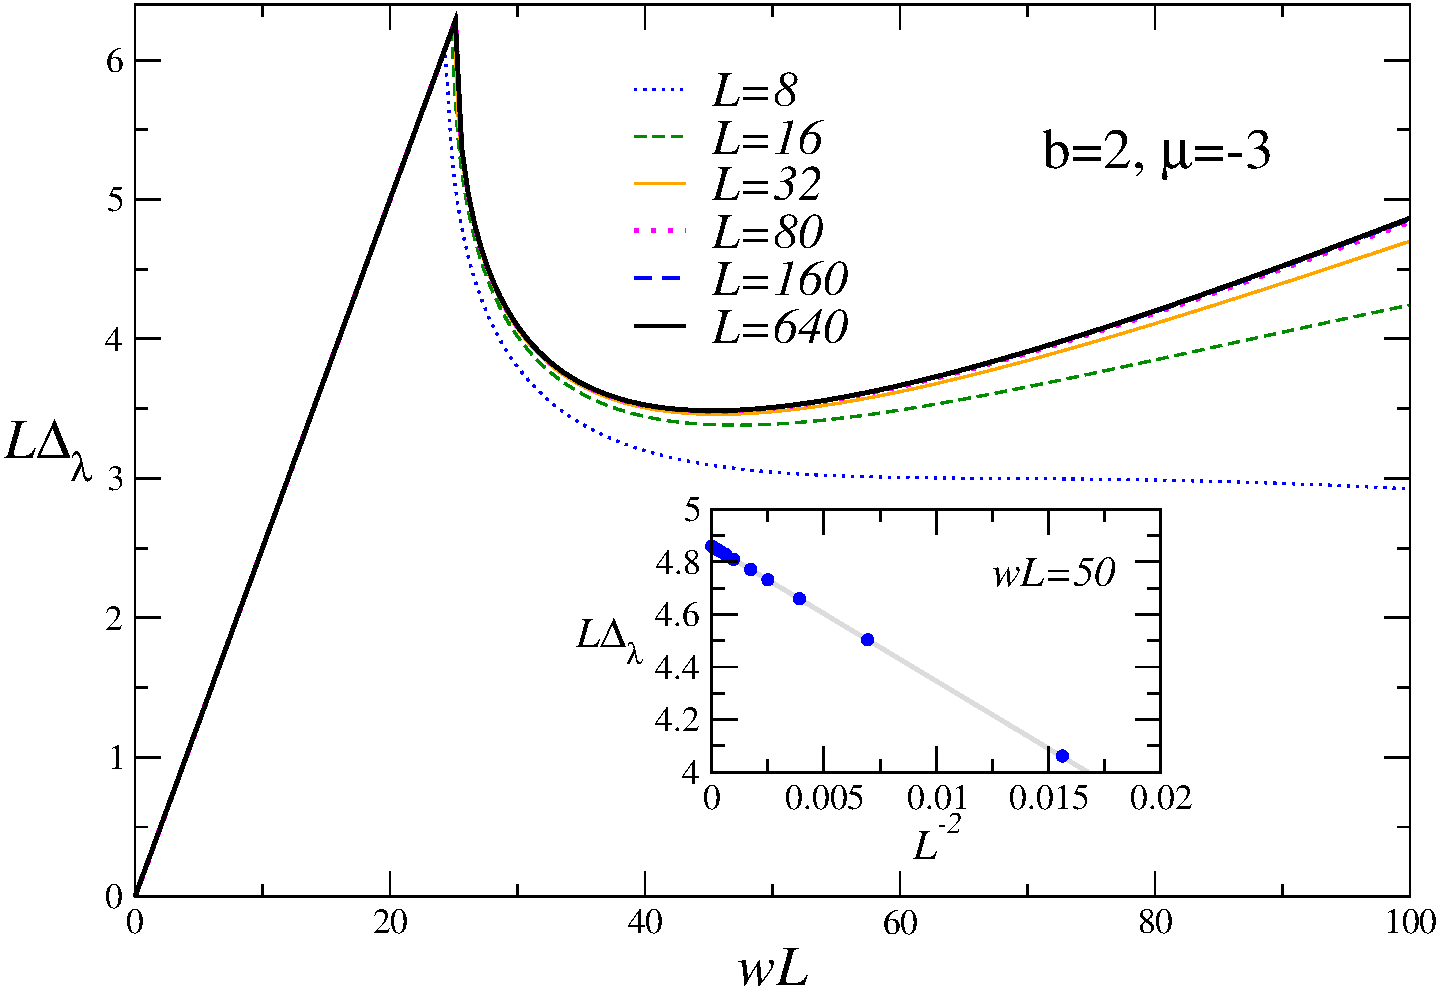
\includegraphics[width=8cm]{imm/scalingDeltaapbc.pdf}
    \label{fig_ratelatetime}
\end{figure}

\end{frame}

\begin{frame}
	\frametitle{Liouvillian gap $n$ fixed}
\begin{figure}[!b]
    \centering
    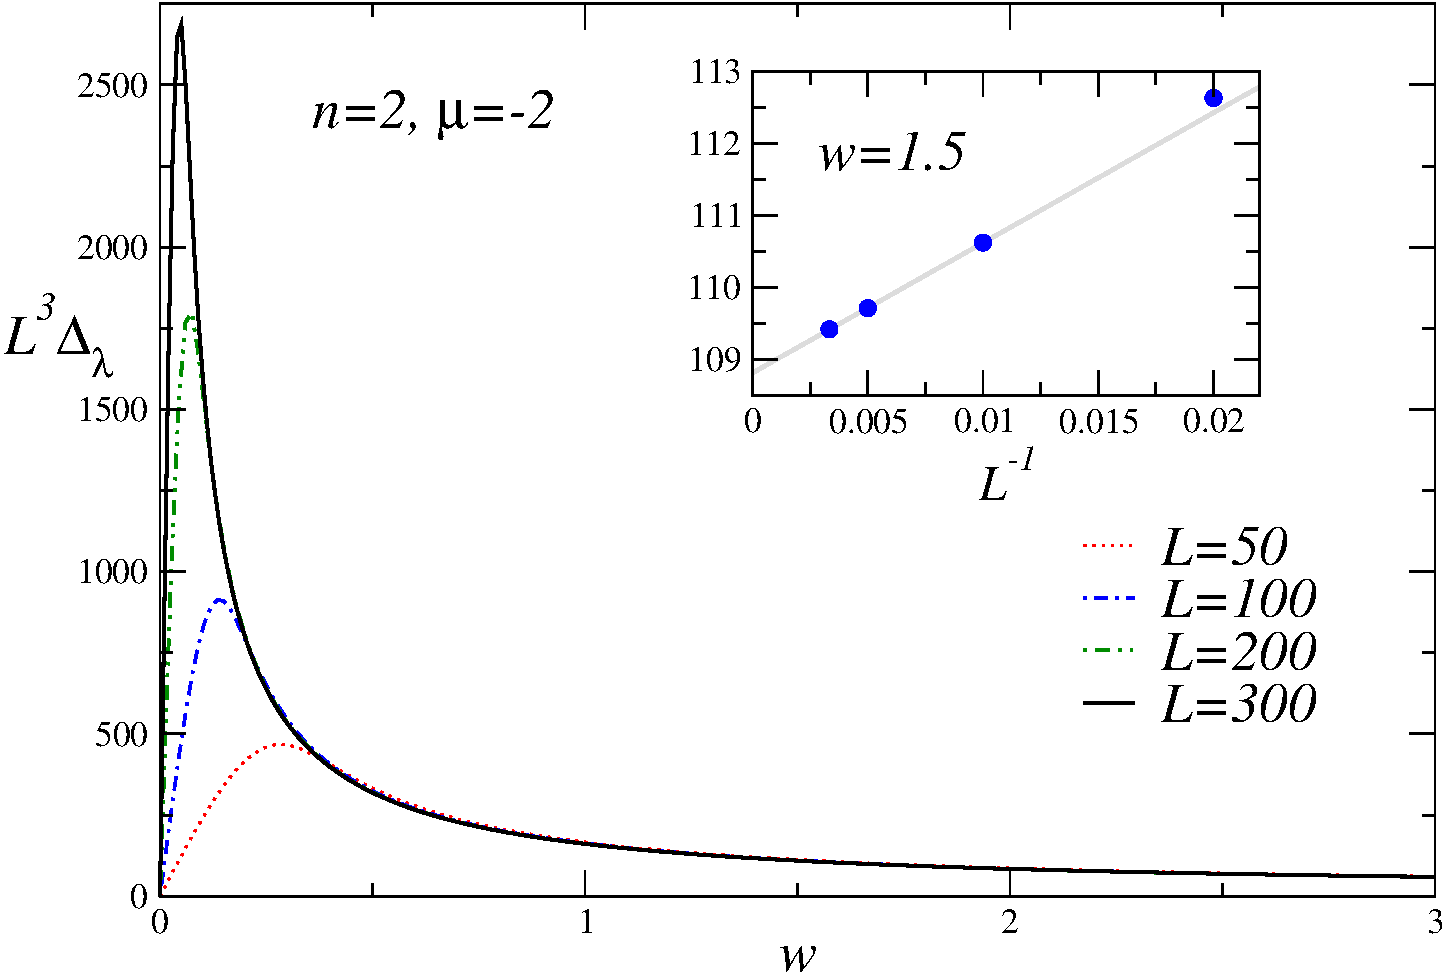
\includegraphics[width=6.4cm]{imm/delantipk0bl2L3Dw.pdf}
    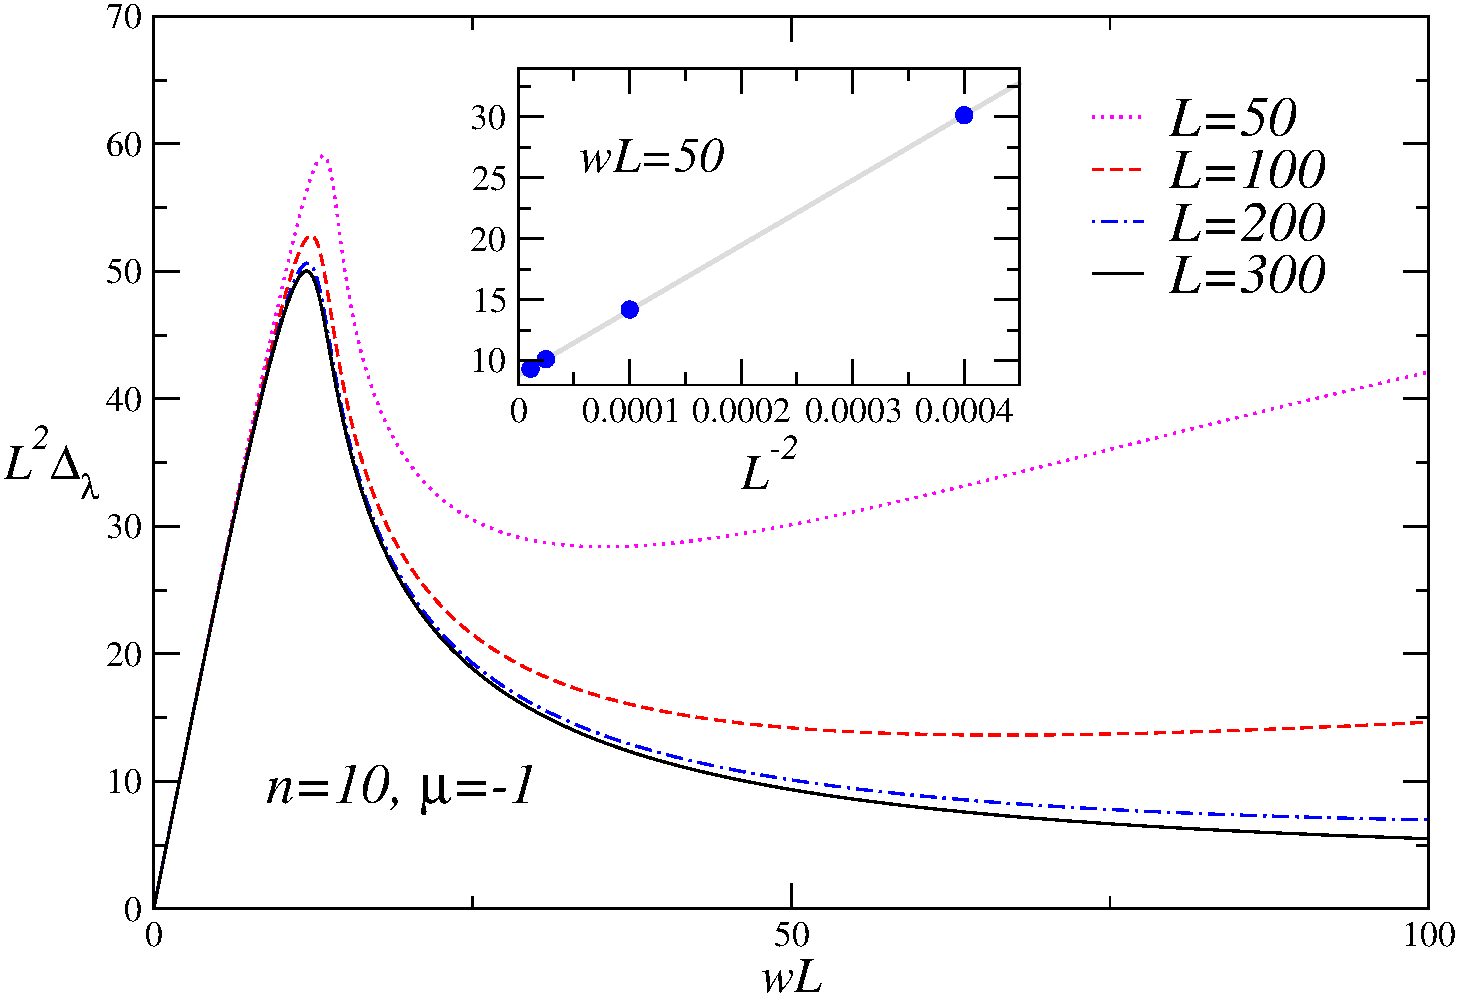
\includegraphics[width=6.4cm]{imm/scalingDeltanfixedmuminus1.pdf}
	\label{fig_scaling_delta_apbc}
\end{figure}

\end{frame}

\begin{frame}
	\frametitle{Dynamic Finite Size Scaling}
	The correlation function as observable:
	\begin{align}
        C(x, y, t)&\equiv{\rm Tr}[\rho(t)(\hat{c}^\dagger_x\hat{c}_y+\hat{c}^\dagger_y\hat{c}_x)]\,,\\
        P(x, y, t)&\equiv{\rm Tr}[\rho(t)(\hat{c}^\dagger_x\hat{c}^\dagger_y+\hat{c}_y\hat{c}_x)]\,.
    \label{eq_def_two_point_functions_C_P}
	\end{align}


	The scaling parameters are set:
	\ba{}
	M_{i/f}=(\mu_{i/f}-\mu_c)L^{y_\mu} &\qquad y_\mu = 1 \pc \\
	\Theta = t L^{-z}\,,\,\, z=1 \,\, 
	{\rm for} \,\, t \sim L &\pc \qquad
	\Theta = t /\Delta_\lambda \,\, 
	{\rm for} \,\, t\sim L^3 \pc \\
	\gamma_b=\frac{wL^{z}}{b}\,& \,\,.
	\ea


	The Scaling Laws can be expressed:
	\begin{align}
    C(x, y, t) &\approx L^{-2y_c}\mathcal{C}(M_i, M_f, \{X_i\}, \Theta, \gamma_b) \,\, ,   \notag \\
    P(x, y, t) &\approx L^{-2y_c}\mathcal{P}(M_i, M_f, \{X_i\}, \Theta, \gamma_b)\,.\notag
\end{align}

\end{frame}

\begin{frame}
	\frametitle{Numerical Results}
	\begin{figure}
    \centering
    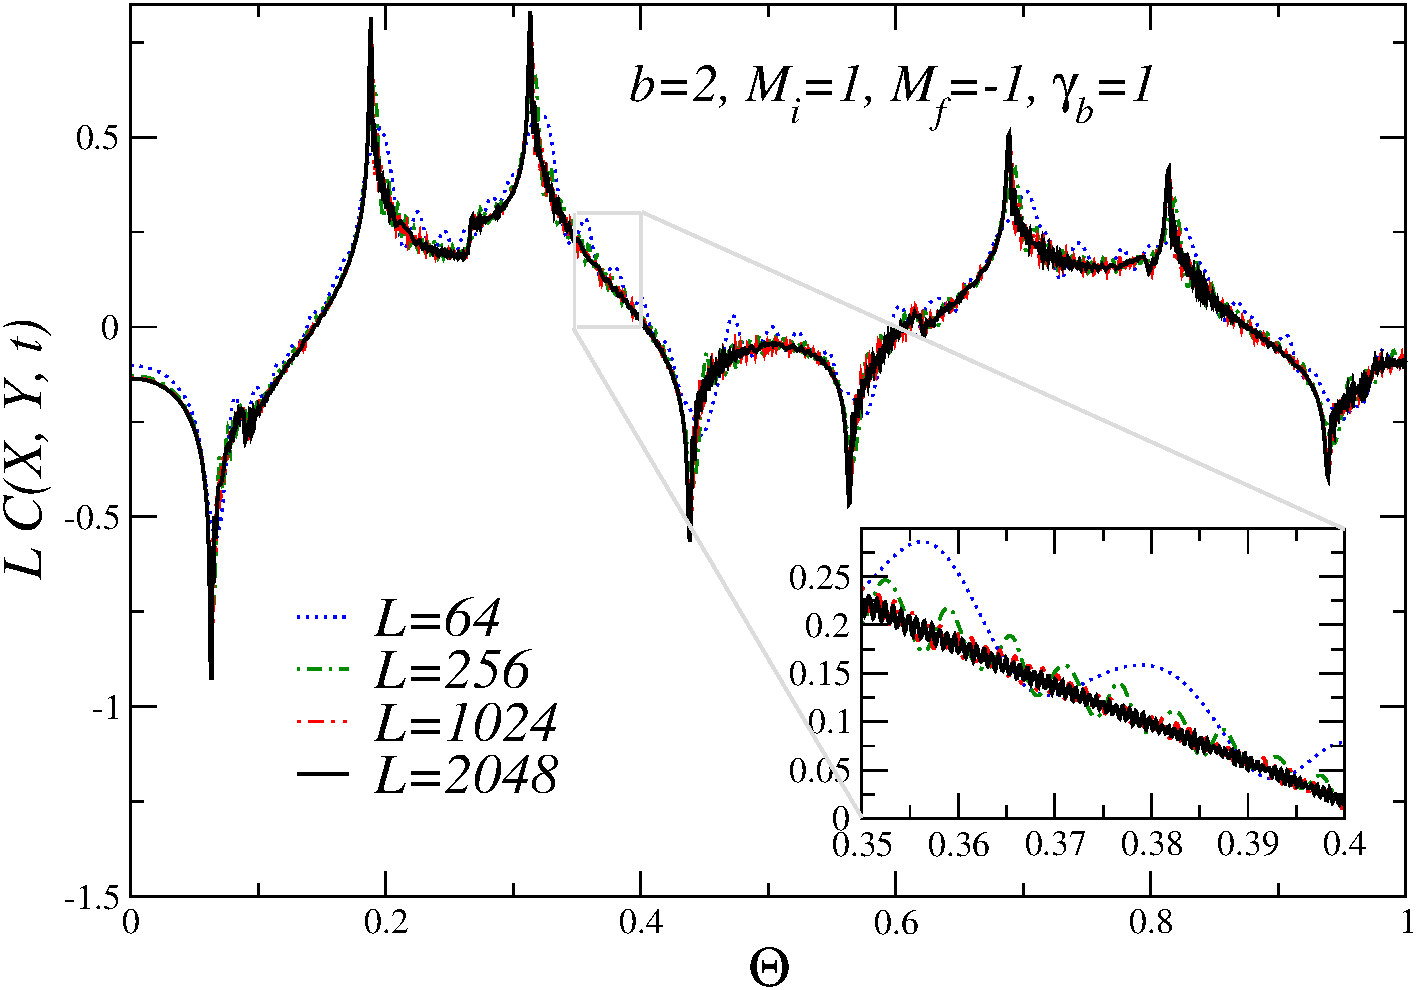
\includegraphics[width=6.4cm]{imm/Cscaling2b.pdf}
    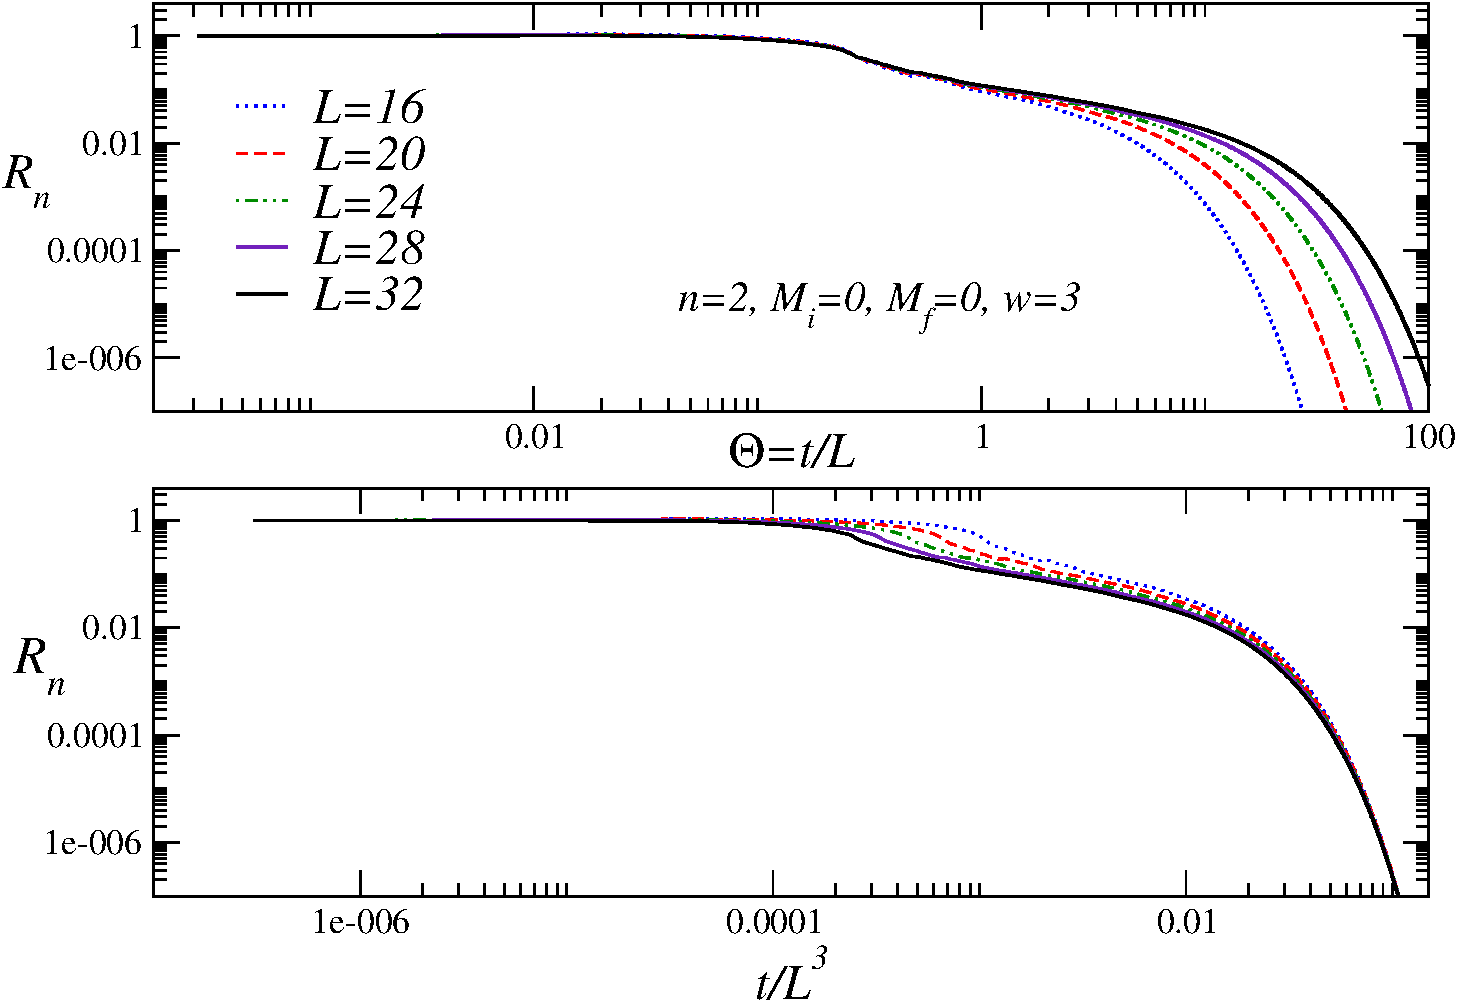
\includegraphics[width=6.4cm]{imm/fss_and_gap_n_fixed.pdf}
    \label{fig_Cscaling2b}
\end{figure}
We introduce the RG invariant quantity $R_n$ defined as 
\begin{equation}
    R_n = \frac{N(t) - N_{\text{asy}}}{N(0) - N_{\text{asy}}}\,,
    \label{def_Rn}
\end{equation}
where $N(t)=\sum_x^L\langle\hat c^\dagger_x \hat c_x(t)\rangle$
and $N_{\text{asy}}=\lim_{t\to\infty}N(t)$. 

\end{frame}

   \section{Conclusions}

\begin{frame}
	\frametitle{Conclusions}
	{\bf In the round-trip model:}
	\begin{itemize}
      	\item
      		Analogy of the scaling behaviors at classical and quantum transitions 
      		is only partially extended to round-trip KZ protocols. 
      		Substantial differences emerge:
      		\begin{enumerate} 
      			\item
      				classical systems develop scaling hysteresis-like scenarios, 
      			\item
      				in quantum systems, the persistence of oscillating relative 
      				phases make the return way extremely sensitive to the 
      				parameters of the protocol;
		\end{enumerate}
		
      	\medskip
      	\medskip

      	\item
      		Even in the simple two-level quantum model, we have a similar 
      		behavior.
      \end{itemize}
      
      \medskip
      \medskip
      \medskip
      
      {\bf In the dissipation scenario:}
      \begin{itemize}
      	\item
      		When we keep $b$ fixed, the gap $\Delta_\lambda$ is always finite
      		 and depends linearly on the dissipation strength $w \pc$ 
      	\medskip
      	\medskip
      	\item 			
      		 Two different regimes: 
      		 \begin{enumerate}
      		 	\item In the small $w$ region, the gap is given by 
      		 	$\Delta_\lambda = w/(2b) \pc$

			\item At large $w$ and sufficiently large $b$,
			$\Delta_\lambda = wC_\mu /b^3$ controls the gap
			in the large-size limit and the dynamic FSS.
		\end{enumerate}

      \end{itemize}

\end{frame}


\end{document}
